%%%%%%%%%%%%%%%%%%%%%%%%%%%%%%%%%%%%%%%%%%%%%%%%%%
% Set document class
\documentclass[12pt]{article}

% Define packages
\usepackage{hyperref, url} 
\usepackage{graphicx,amsfonts,psfrag,layout,subcaption,array,longtable,lscape,booktabs,dcolumn,amsmath,amssymb,amssymb,amsthm,setspace,epigraph,chronology,color,colortbl,caption,wasysym,diagbox,natbib,colortbl,authblk,commath}
\usepackage[]{graphicx}\usepackage[]{color}
\usepackage[page]{appendix}
\usepackage[section]{placeins}
\usepackage[linewidth=1pt]{mdframed}
\usepackage[margin={1in}]{geometry} %1 inch margins

\title{State-Building through Public Land Disposal? An Application of Matrix Completion for Counterfactual Prediction} 
\author[ ]{Jason Poulos\thanks{\emph{Address for correspondence:} Department of Political Science, 210 Barrows Hall \#1950, Berkeley, CA 94720-1950. \emph{Email:} \href{mailto:poulos@berkeley.edu}{\nolinkurl{poulos@berkeley.edu}}. I thank Sean Gailmard, Eric Schickler, Ross Mattheis, and Shom Mazumder for helpful comments. I acknowledge support of the National Science Foundation Graduate Research Fellowship (DGE 1106400). This work used the computer resources of Stampede2 at the Texas Advanced Computing Center (TACC) under an Extreme Science and Engineering Discovery Environment (XSEDE) startup allocation (TG-SES180010).}}
\affil[ ]{University of California, Berkeley}
\date{}
\setcounter{Maxaffil}{0}
\renewcommand\Affilfont{\itshape\small}

% Reference labels in the online appendix
\usepackage{xr}
\externaldocument{land-reform-sm}

% Footnotes stick at the bottom
\usepackage[bottom]{footmisc}

% Multicolumns for references

\usepackage{multicol}

% New footnote characters
\usepackage{footmisc}
\DefineFNsymbols{mySymbols}{{\ensuremath\dagger}{\ensuremath\ddagger}\S\P
   *{**}{\ensuremath{\dagger\dagger}}{\ensuremath{\ddagger\ddagger}}}
\setfnsymbol{mySymbols}

%Rm thanks dagger
\renewcommand\footnotemark{}
%\renewcommand\footnoterule{}

% New tabular environment
\usepackage{tabularx}
\newcolumntype{Y}{>{\raggedleft\arraybackslash}X}% raggedleft column X

% Define appendix 
\renewcommand*\appendixpagename{Appendix}
\renewcommand*\appendixtocname{Appendix}

% Position floats
\renewcommand{\textfraction}{0.05}
\renewcommand{\topfraction}{0.95}
\renewcommand{\bottomfraction}{0.95}
\renewcommand{\floatpagefraction}{0.35}
\setcounter{totalnumber}{5}

% Colors for highlighting tables
\definecolor{Gray}{gray}{0.9}

% Different font in captions
\newcommand{\captionfonts}{\scriptsize}

\makeatletter  % Allow the use of @ in command names
\long\def\@makecaption#1#2{%
  \vskip\abovecaptionskip
  \sbox\@tempboxa{{\captionfonts #1: #2}}%
  \ifdim \wd\@tempboxa >\hsize
    {\captionfonts #1: #2\par}
  \else
    \hbox to\hsize{\hfil\box\@tempboxa\hfil}%
  \fi
  \vskip\belowcaptionskip}
%\makeatother   % Cancel the effect of \makeatletter
 
% Set Spacing
\doublespacing

% Number assumptions
\newtheorem*{assumption*}{\assumptionnumber}
\providecommand{\assumptionnumber}{}
\makeatletter
\newenvironment{assumption}[2]
 {%
  \renewcommand{\assumptionnumber}{Assumption #1}%
  \begin{assumption*}%
  \protected@edef\@currentlabel{#1}%
 }
 {%
  \end{assumption*}
 }
\makeatother

% Macros
\newcommand{\Adv}{{\mathbf{Adv}}}       
\newcommand{\prp}{{\mathrm{prp}}}                  % How to define new commands 
\newcommand{\calK}{{\cal K}}
\newcommand{\outputs}{{\Rightarrow}}                
\newcommand{\getsr}{{\:\stackrel{{\scriptscriptstyle\hspace{0.2em}\$}}{\leftarrow}\:}}
\newcommand{\andthen}{{\::\;\;}}    %  \: \; for thinspace, medspace, thickspace
\newcommand{\Rand}[1]{{\mathrm{Rand}[{#1}]}}       % A command with one argument
\newcommand{\Perm}[1]{{\mathrm{Perm}[{#1}]}}       
\newcommand{\Randd}[2]{{\mathrm{Rand}[{#1},{#2}]}} % and with two arguments
\newcommand{\E}{\mathrm{E}}
\newcommand{\Var}{\mathrm{Var}}
\newcommand{\Cov}{\mathrm{Cov}}
\DeclareMathOperator*{\plim}{plim}
\newcommand\independent{\protect\mathpalette{\protect\independenT}{\perp}}
\def\independenT#1#2{\mathrel{\rlap{$#1#2$}\mkern2mu{#1#2}}}
\newcommand{\possessivecite}[1]{\citeauthor{#1}'s (\citeyear{#1})} 

%%%%%%%%%%%%%%%%%%%%%%%%%%%%%%%%%%%%%%%%%%%%%%%%%%%%%%%%%%%%%%%%%%%%%%%%%%%%

\begin{document} 
 
\begin{singlespacing}
\maketitle  
\end{singlespacing}

\thispagestyle{empty}
%\pagenumbering{roman}% Roman-numbered pages (start from i)

%\pagebreak % abstract/keywords get own page 
\begin{abstract}  
\noindent
How would the frontier have evolved in the absence of mid-nineteenth century homestead policies? I propose using matrix completion --- a machine learning method commonly used for recommendation tasks --- to predict the counterfactual time-series of frontier state capacity had there been no homesteading. The matrix completion method outperforms several linear regression-based estimators in placebo tests. Time-specific causal estimates signify that homestead policies had significant and long-lasting negative impacts on state government expenditure and revenue. These results are consistent with difference-in-difference estimation that exploits variation in the timing and intensity of homestead entries aggregated from 1.46 million individual land patents.\\
%\vspace{10mm}
%\emph{Keywords:} causal inference; machine learning; state capacity; synthetic control method; time-series prediction
\end{abstract}	

%Move introduction to second page
\pagebreak
\pagenumbering{arabic}% Arabic-numbered pages (start from 1)

Political scientists are increasingly interested in patterns of state development across time and place. Several scholars \citep[e.g.,][]{bensel1990,murtazashvili2013political,frymer2014rush} theorize a relationship between mid-nineteenth century public land policies and the development of the U.S. government, arguing that policies designed to transfer public land to private individuals increased the bureaucratic capacity of the federal government to administer land. 

Public land policies had long-lasting impacts on state capacity, or the ability of state governments to finance and implement policies \citep{besley2010state}. I explore the role of two major land policies in shaping state capacity: the Homestead Act (HSA) of 1862, which opened for settlement hundreds of millions of acres of western frontier land, and the Southern Homestead Act (SHA) of 1866, which opened over 46 million acres of land for homesteading. I provide evidence that homesteads authorized under these laws had long-run positive impacts on the capacity of frontier state governments. 

The view that the western frontier had long-lasting impacts on the evolution of democratic institutions can be traced to \citet{turner1956significance}. Turner's ``frontier thesis" posited that homestead policies acted as a ``safety valve'' for relieving pressure from congested urban labor markets in eastern states. The view of the frontier as a ``safety valve'' has been explored by \citet{ferrie1997migration}, who finds evidence in a linked census sample of substantial migration to the frontier by unskilled workers and considerable gains in wealth for these migrant workers. Homestead policies not only offered greater economic opportunities to eastern migrants, but also the scarcity of people on the western frontier meant that state and local governments competed with each other to attract migrants in order to lower local labor costs and to increase land values and tax revenues \citep{engerman2005evolution}. Frontier governments offered migrants broad access to cheap land and property rights, unrestricted voting rights, and a more generous provision of schooling and other public goods.%\footnote{\citet{engerman2005evolution} note that the commitment of frontier state governments to offer greater political and economic opportunities for migrants was more prevalent in western states than in the South.}

\citet{garcia2009myth} test the frontier thesis in a global context and conclude that the economic effect of the frontier depends on the quality of political institutions at the time of frontier expansion: frontier expansion promoted equitable outcomes only when societies were initially democratic; however, when institutional quality is weak, the existence of frontier land can yield worse development outcomes because non-democratic political elites can consolidate frontier lands for themselves. Historical scholars have noted that public land policies were often exploited by land speculators, ranchers, miners, and loggers, to accumulate public land and extract natural resources during the early stages of capitalist development \citep{gates1942role,murtazashvili2013political}. According to this view, homesteading laws were \emph{de jure} social polices but \emph{de facto} corporate welfarism. 

The paper makes a methodological contribution in applying an alternative method for estimating causal impacts of policy interventions on time-series cross-sectional data. Building on a new literature that uses machine learning algorithms such as L1-regularized linear regression \citep{doudchenko2016balancing} or deep neural networks \citep{poulos2017rnn} for counterfactual prediction, I apply a matrix completion method to predict the treated unit time-series in the absence of the intervention. I perform placebo tests and find that the matrix completion method outperforms the synthetic control method and other regression-based estimators in terms of minimizing prediction error. In addition, I show how to evaluate the overall effect of the policy intervention using a randomization inference procedure in which approximately unbiased $p$-values are obtained under minimal assumptions by permuting the time-series dimension of the data under the null.

The paper proceeds as follows: in Section \ref{history}, I overview the historical context of homestead policies and its relationship to state capacity and land inequality; Section \ref{estimation} describes the method of matrix completion for counterfactual prediction, benchmarks the method against the synthetic control method and alternative estimators, and describes the inferential procedure. In Section \ref{state-capacity}, I report the results of placebo tests to verify the consistency of the matrix completion estimator and present estimates of the long-run impacts of homestead policies on state capacity. Section~\ref{DID} reports DID estimates of the effect of homesteads on state capacity and land inequality, and Section~\ref{discussion} concludes. 

\setcounter{section}{1} % intro is 1
\section{Historical background} \label{history}

The 1862 HSA opened up hundreds of millions of acres of western public land for settlement. The HSA provides that any adult citizen --- including women, immigrants who had applied for citizenship, and freed slaves following the passage of the Fourteenth Amendment---  could apply for a homestead grant of 160 acres of frontier land. Applicants were required to live and make improvements on the land for five years before filing to claim a homestead land grant. The explicit goal of the HSA was to liberalize the homesteading requirements set by the Preemption Act of 1841, which permitted individuals already inhabiting public land to purchase up to 160 acres at \$1.25 per acre before the land was put up for sale. The implicit goal was to promote rapid settlement on the western frontier and reduce federal government's enforcement costs \citep{allen1991homesteading}. Under the HSA, the bulk of newly surveyed land on the western frontier was reserved for homesteads, although the law did not end sales of public land.\footnote{Congress repealed the cash entry restriction in 1876, and sharply reversed policy in 1889 by ending cash entry in all PLS except for Missouri \citep{gates1940federal}.}

In the pre-Reconstruction South, public land was not open to homestead but rather unrestricted cash entry, which permitted the direct sale of public land to private individuals of 80 acres or more for at least \$1.25 an acre. The 1866 SHA restricted cash entry and reserved for homesteading over 46 million acres of public land, or about one-third of the total land area in the five southern public land states (PLS) \citep[pp. 13]{lanza1999agrarianism}. Note that I use the terminology of PLS interchangeably with ``frontier" states throughout the paper. PLS are states created out of the public domain. In the South, these states include Alabama, Arkansas, Florida, Louisiana, and Mississippi. Western PLS include the 25 states that comprise the Midwestern, Southwestern, and Western U.S. (except Hawaii). Similar to the HSA, homesteaders could patent up to 160 acres after five years of inhabiting and improving the land, but unlike the HSA, could not commute homestead entries to cash entry after six months.%  In sum, the SHA followed the same application procedures as the HSA but differed in that it restricted cash sales of public land for the decade after its passage. 

Homestead policies may have failed to create a more equitable land distribution in part due to the accumulation of public land by speculators and corporations through corrupt practices, such as the use of dummy entry-men, which is the practice of paying individuals to stake out a homestead in order to extract resources from the land with no intention of filing for the final patent. In the South, dummy entry-men were used by timber and mining companies to extract resources while the cash entry restriction of the SHA was in effect. When the restriction was removed, there was no need for fraudulent filings because the larger companies could buy land in unlimited amounts at a nominal price \citep{gates1940federal, gates1979federal}. The same pattern of fraudulent filings existed in the West, where \citet{murtazashvili2013political} argues that speculators benefited disproportionately from public land policies because the economic balance of power tilted toward the wealthy. \citet{gates1942role} characterizes western speculators who bought land in bulk prior to the 1889 restriction as being influential in state and local governments, resistant to paying taxes, and opposed to expenditures except for transportation facilities close to their land. 

\section{Matrix completion for counterfactual prediction} \label{estimation}

An important problem in the social sciences is estimating the effect of a binary intervention on an outcome over time. When interventions take place at an aggregate level (e.g., a state), researchers make causal inferences by comparing the post-intervention outcomes of affected (``treated'') units against the outcomes of unaffected  (``control'') units. In the current application, PLS are the treated units and state land states (SLS) --- i.e., states that were not crafted from the public domain and were therefore not directly affected by homestead policies --- serve as control units.\footnote{SLS includes states of the original 13 colonies, Maine, Tennessee, Texas, Vermont, and West Virginia.} A common approach to the problem is the synthetic control method, which predicts the counterfactual outcomes for treated units by finding a convex combination of control units that match the treated units in term of lagged outcomes. The synthetic control method predicts patterns across units that are assumed to remain constant over time. 

This paper applies the  method of matrix completion via nuclear norm minimization (MC-NNM) proposed by \citet{athey2017matrix} to predict counterfactual outcomes in a setting where multiple treated units are exposed to a binary intervention and the date of initial exposure to treatment may vary between treated units.\footnote{\citet{schnabel2016recommendations} first connected the matrix completion problem with causal inference in an observational setting in the context of recommender systems under selection bias.} Matrix completion methods \citep[e.g.,][]{mazumder2010spectral} exploit correlations within and across units, but ignore the temporal dimension of the data and typically assume missing values are sampled uniformly at random \citep{yoon2018estimating}. In contrast, the MC-NNM estimator allows for patterns of missing data in $\mathbf{Y}$ to have a time-series dependency structure that arise from simultaneous or staggered adoption.

Let $\mathbf{Y}$ denote a $N \times T$ matrix of outcomes for each unit $i, \ldots, N$ at time $t = 1, \ldots, T$. $\mathbf{Y}$ is incomplete because we observe each element $Y_{it}$ for only the control units and the treated units prior to first treatment exposure. Let $\mathcal{O}$ denote the set of $(it)$ values that are observed and $\mathcal{M}$ the set of missing values. Define the $N \times T$ complete matrix $\mathbf{M}$, where $M_{it} =1 $ if $(it) \in \mathcal{M}$ and $M_{it} = 0$ if $(it) \in \mathcal{O}$ is nonmissing.\footnote{The process that generates $\mathbf{M}$ is referred to the assignment mechanism in the causal inference literature \citep{imbens2015causal} and the missing data mechanism in missing data analysis \citep{little2014}.} This setup is motivated by the fundamental problem of causal inference \citep{holland1986statistics} in that we cannot directly observe counterfactual outcomes and we instead wish to impute missing values in $\mathbf{Y}$ for treated units with $M_{it}=1$. 

In an observational setting, units are part of the assignment mechanism that generates $\mathbf{M}$ and patterns of missing data follow one of two specific structures. In the case of simultaneous adoption of treatment, a subset of units are exposed to treatment at time $T_0$ and every subsequent period. The second structure arises from staggered adoption, which differs from simultaneous adoption in that $T_0$ may vary across treated units. In either case, there are selection biases because the probability of missingness may depend on the unobserved data. Selection bias in the staggered adoption setting can occur in the current application if PLS are exposed to treatment (i.e., settled homesteads) earlier because they have higher quality land. The goal is to accurately estimate the effect of a policy intervention despite incomplete data subject to selection bias. 

\subsection{Matrix completion estimator}

Matrix completion methods attempt to impute missing entries in a low-rank matrix by solving a convex optimization problem via nuclear norm minimization, even when relatively few values are observed in the full matrix $\mathbf{Y}$ \citep{candes2009exact,candes2010matrix}. Low-rank matrices arise in the present context when only a few factors contribute to the outcomes. The MC-NNM estimator is 

\begin{equation}
Y_{it} = L_{it}^{*} + \sum_{p=1}^{P} X_{ip} \beta^{*} + \gamma_{i}^{*} + \delta_{t}^{*} + \epsilon_{it} \label{eq:mc-Y}
\end{equation}

\noindent
where $\mathbf{L^{*}}$ a low-rank matrix to be estimated, $\mathbf{X}$ is a $N \times P$ matrix of normalized unit-specific covariates, and $\gamma^{*}$ and $\delta^{*}$ are unit and time effects, respectively. The identifying condition is that, conditional on $\mathbf{L^{*}}$, the error term $\epsilon$ is independent across rows (units) and $\E[\epsilon | \mathbf{L^{*}} + \beta^{*} + \gamma^{*} + \delta^{*}] = 0$. Estimating $\mathbf{L^{*}}$ involves minimizing the sum of squared errors via nuclear norm regularized least squares:

\begin{equation}
\min_{\mathbf{L}, \beta} \Bigg[\sum_{(it) \in \mathcal{O}} \frac{1}{|\mathcal{O}|} \bigg(Y_{it} - L_{it} - \sum_{p=1}^{P} X_{ip} \beta - \gamma_{i} - \delta_{t} \bigg)^2 + \lambda \norm{\mathbf{L}}_\star \Bigg], \label{eq:mc-opt}
\end{equation}

\noindent
where $\lambda$ is the regularization term on the nuclear norm $\norm{\cdot}_\star$ (i.e., sum of singular values) that is chosen by cross-validation. The algorithm for (\ref{eq:mc-opt}) iteratively replaces missing values with those recovered from a singular value decomposition (SVD) \citep{mazumder2010spectral}.\footnote{\citet{amjad2018robust} propose an alternative approach of approximating $\mathbf{L^{*}}$ via SVD, and then using linear regression on the ``de-noised'' matrix, rather than relying on matrix norm regularizations.} 

\citet{athey2017matrix} note two drawbacks of the MC-NNM estimator: first, it penalizes the errors for each value with $M_{it} = 0$ equally without regard to the fact that $P(M_{it}) = 1$ (i.e., the propensity score) increases with $t$. Second, the estimator does not account for time-series dependencies in the observed data and therefore it is likely that the columns of $\epsilon$ are autocorrelated.

\subsection{Simulations} \label{sims}

In this section, I evaluate the accuracy of the MC-NNM estimator on the following three datasets common to the synthetic control literature, with the actual treated unit removed from each dataset: \possessivecite{abadie2003economic} study of the economic impact of terrorism in the Basque Country during the late 1960s ($N=16$, $T=43$); \possessivecite{abadie2010synthetic} study of the effects of a large-scale tobacco control program implemented in California in 1988 ($N=38$, $T=31$); and \possessivecite{abadie2015comparative} study of the economic impact of the 1990 German reunification on West Germany ($N=16$, $T=44$). For each trial run, I randomly select half of the control units to be treated and predict their counterfactual outcomes for periods following a randomly selected initial treatment time $T_0$. I compare the predicted values to the observed values by calculating the root-mean squared error (RMSE), $\sum_{it}|\mathbf{L^{*}} -\hat{\mathbf{L}}|^2 / \sqrt{NT}$. 

I benchmarks the MC-NNM estimator against the following previously used estimators:

\begin{description}
	{\setlength\itemindent{1mm}
		\item[DID] Horizontal regression of $\mathbf{Y}$ on unit and time effects and a binary treatment variable \citep{athey2017matrix}
		\item[HR-EN] Horizontal regression with elastic net regularization \citep{athey2017matrix} 
		\item[PCA] Regularized iterative principal components analysis \citep{ilin2010practical}
		\item[SC-ADH] Synthetic control approached via exponentiated gradient descent \citep{abadie2010synthetic}
		\item[SVD] Low-rank SVD approximation estimated by expectation maximization \citep{troyanskaya2001missing}
		\item[VT-EN] The same as HR-EN, but $\mathbf{Y}$ is transposed.
	}
\end{description}

Figure \ref{synth-stag} reports the average prediction error of the estimators in a staggered treatment adoption setting, across different ratios $T_0/T$, where $T_0$ denotes the number of pre-periods. Across all estimators, the average RMSE decreases and confidence bands narrow as $T_0/T$ approaches unity because the estimators have more information to generate counterfactual predictions. The MC-NNM estimator generally outperforms all other estimators in terms of average RMSE across different ratios $T_0/T$.  The strong performance of the MC-NNM estimator can be attributed to the fact that it is capable of using additional information in the form of pre-period observations of the treated units, whereas the regression-based estimators rely only on the pre-intervention observations of control units to predict counterfactuals.\footnote{Figure SM-\ref{synth-sim} in the Supporting Materials (SM) present a similar pattern of results in a simultaneous adoption setting.}

\begin{figure}[htbp]
	\centering
	\begin{subfigure}[t]{0.48\textwidth}
		\centering
		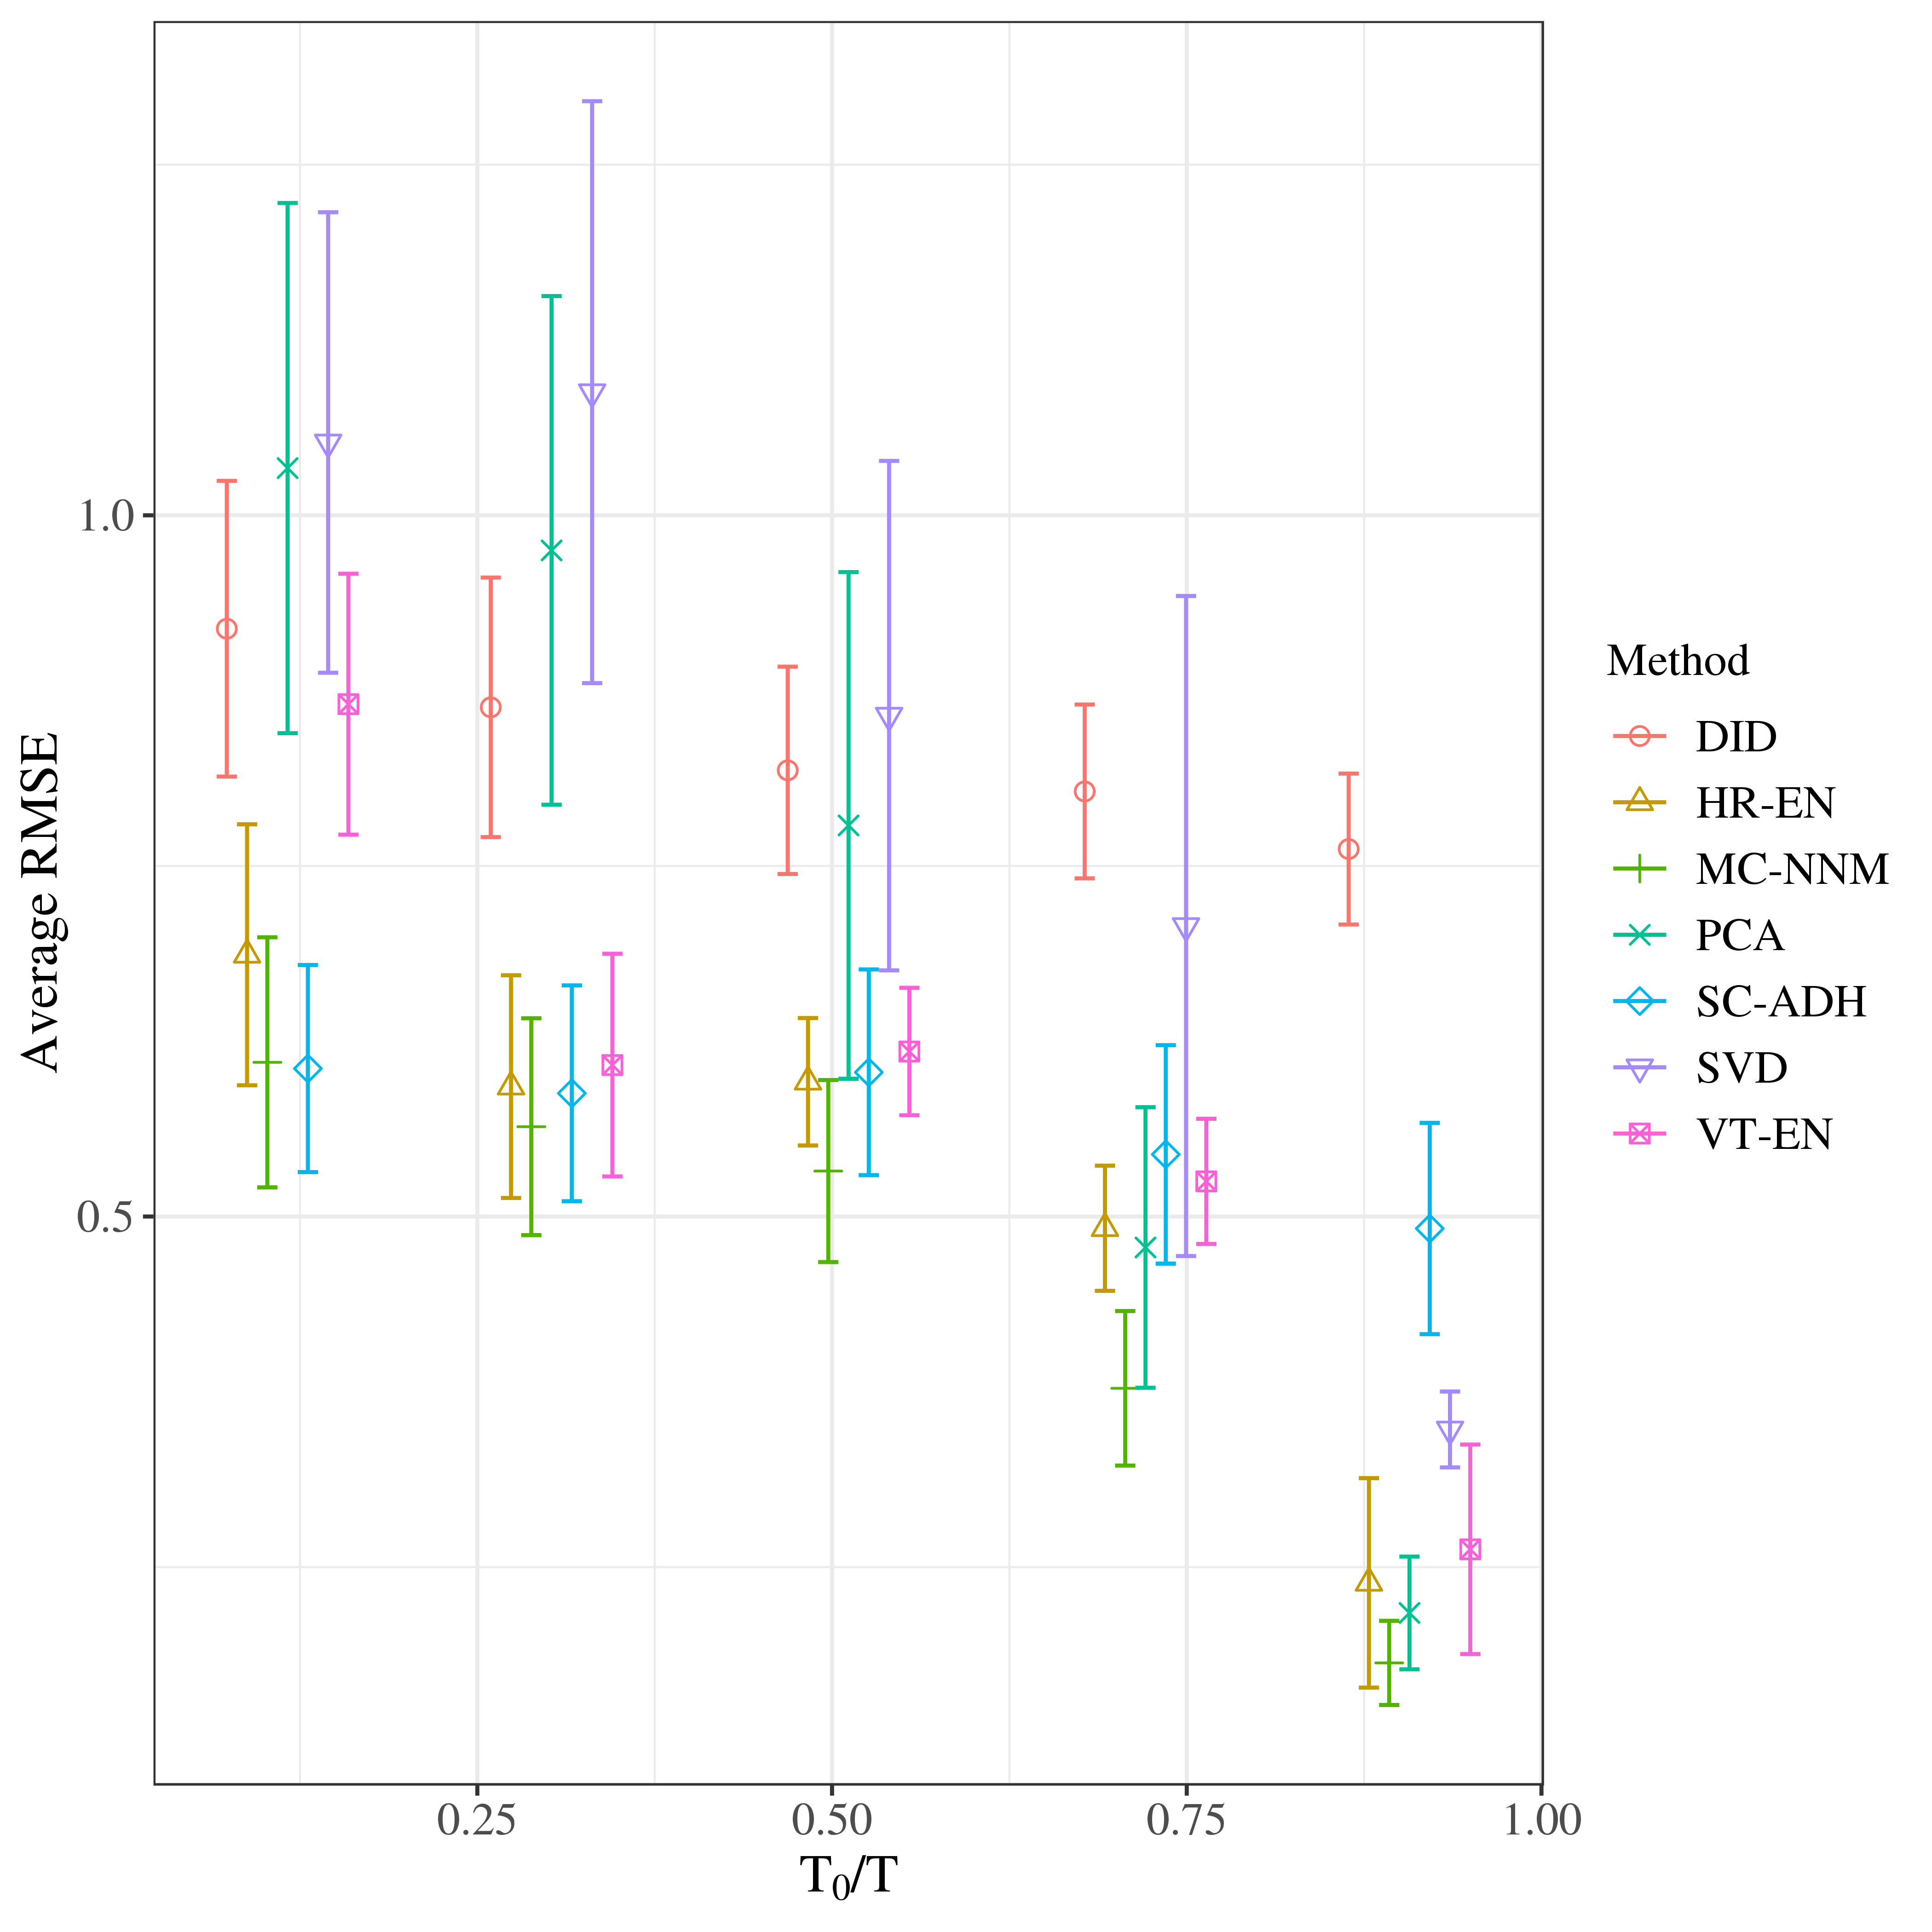
\includegraphics[width=\textwidth]{plots/basque_N_16_T_43_numruns_20_num_treated_8_simultaneuous_0.png}
		\caption{Basque Country terrorism data, $N_t = 8$} 
	\end{subfigure}
	~ 
	\begin{subfigure}[t]{0.48\textwidth}
		\centering
		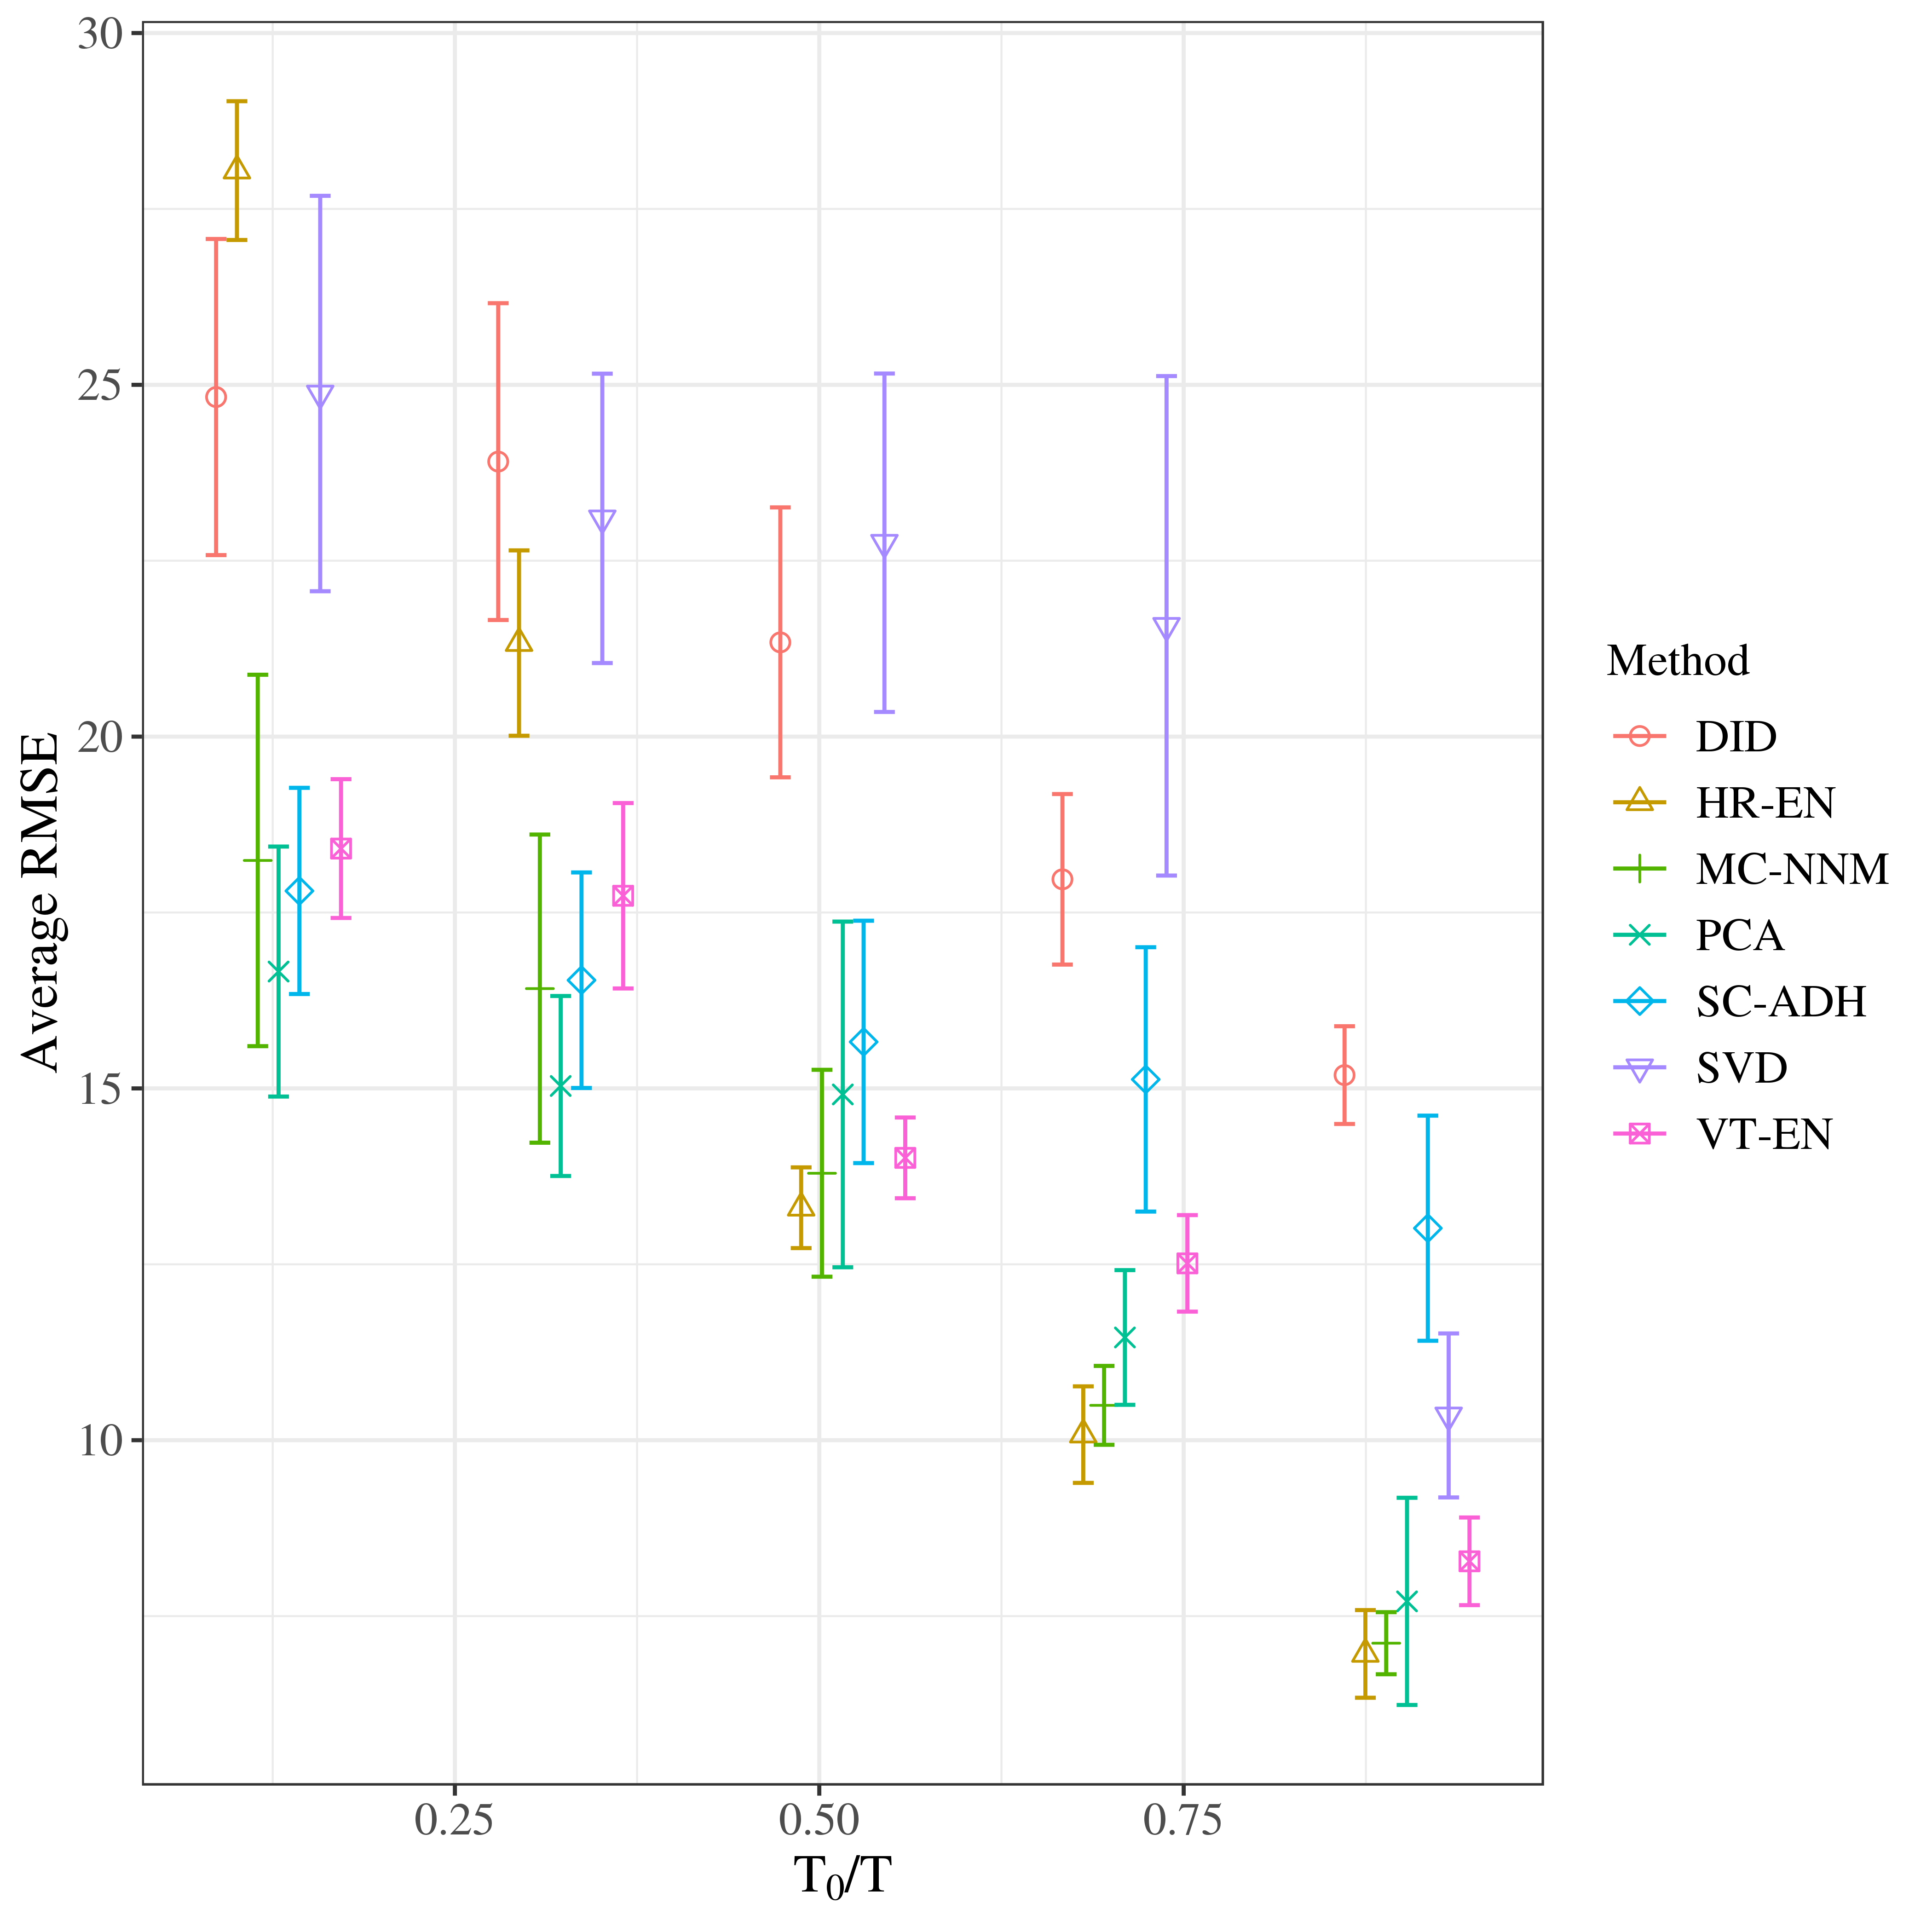
\includegraphics[width=\textwidth]{plots/california_N_38_T_31_numruns_20_num_treated_19_simultaneuous_0.png}
		\caption{California smoking ban data, $N_t = 19$}
	\end{subfigure}
	~ 
	\begin{subfigure}[t]{0.48\textwidth}
		\centering
		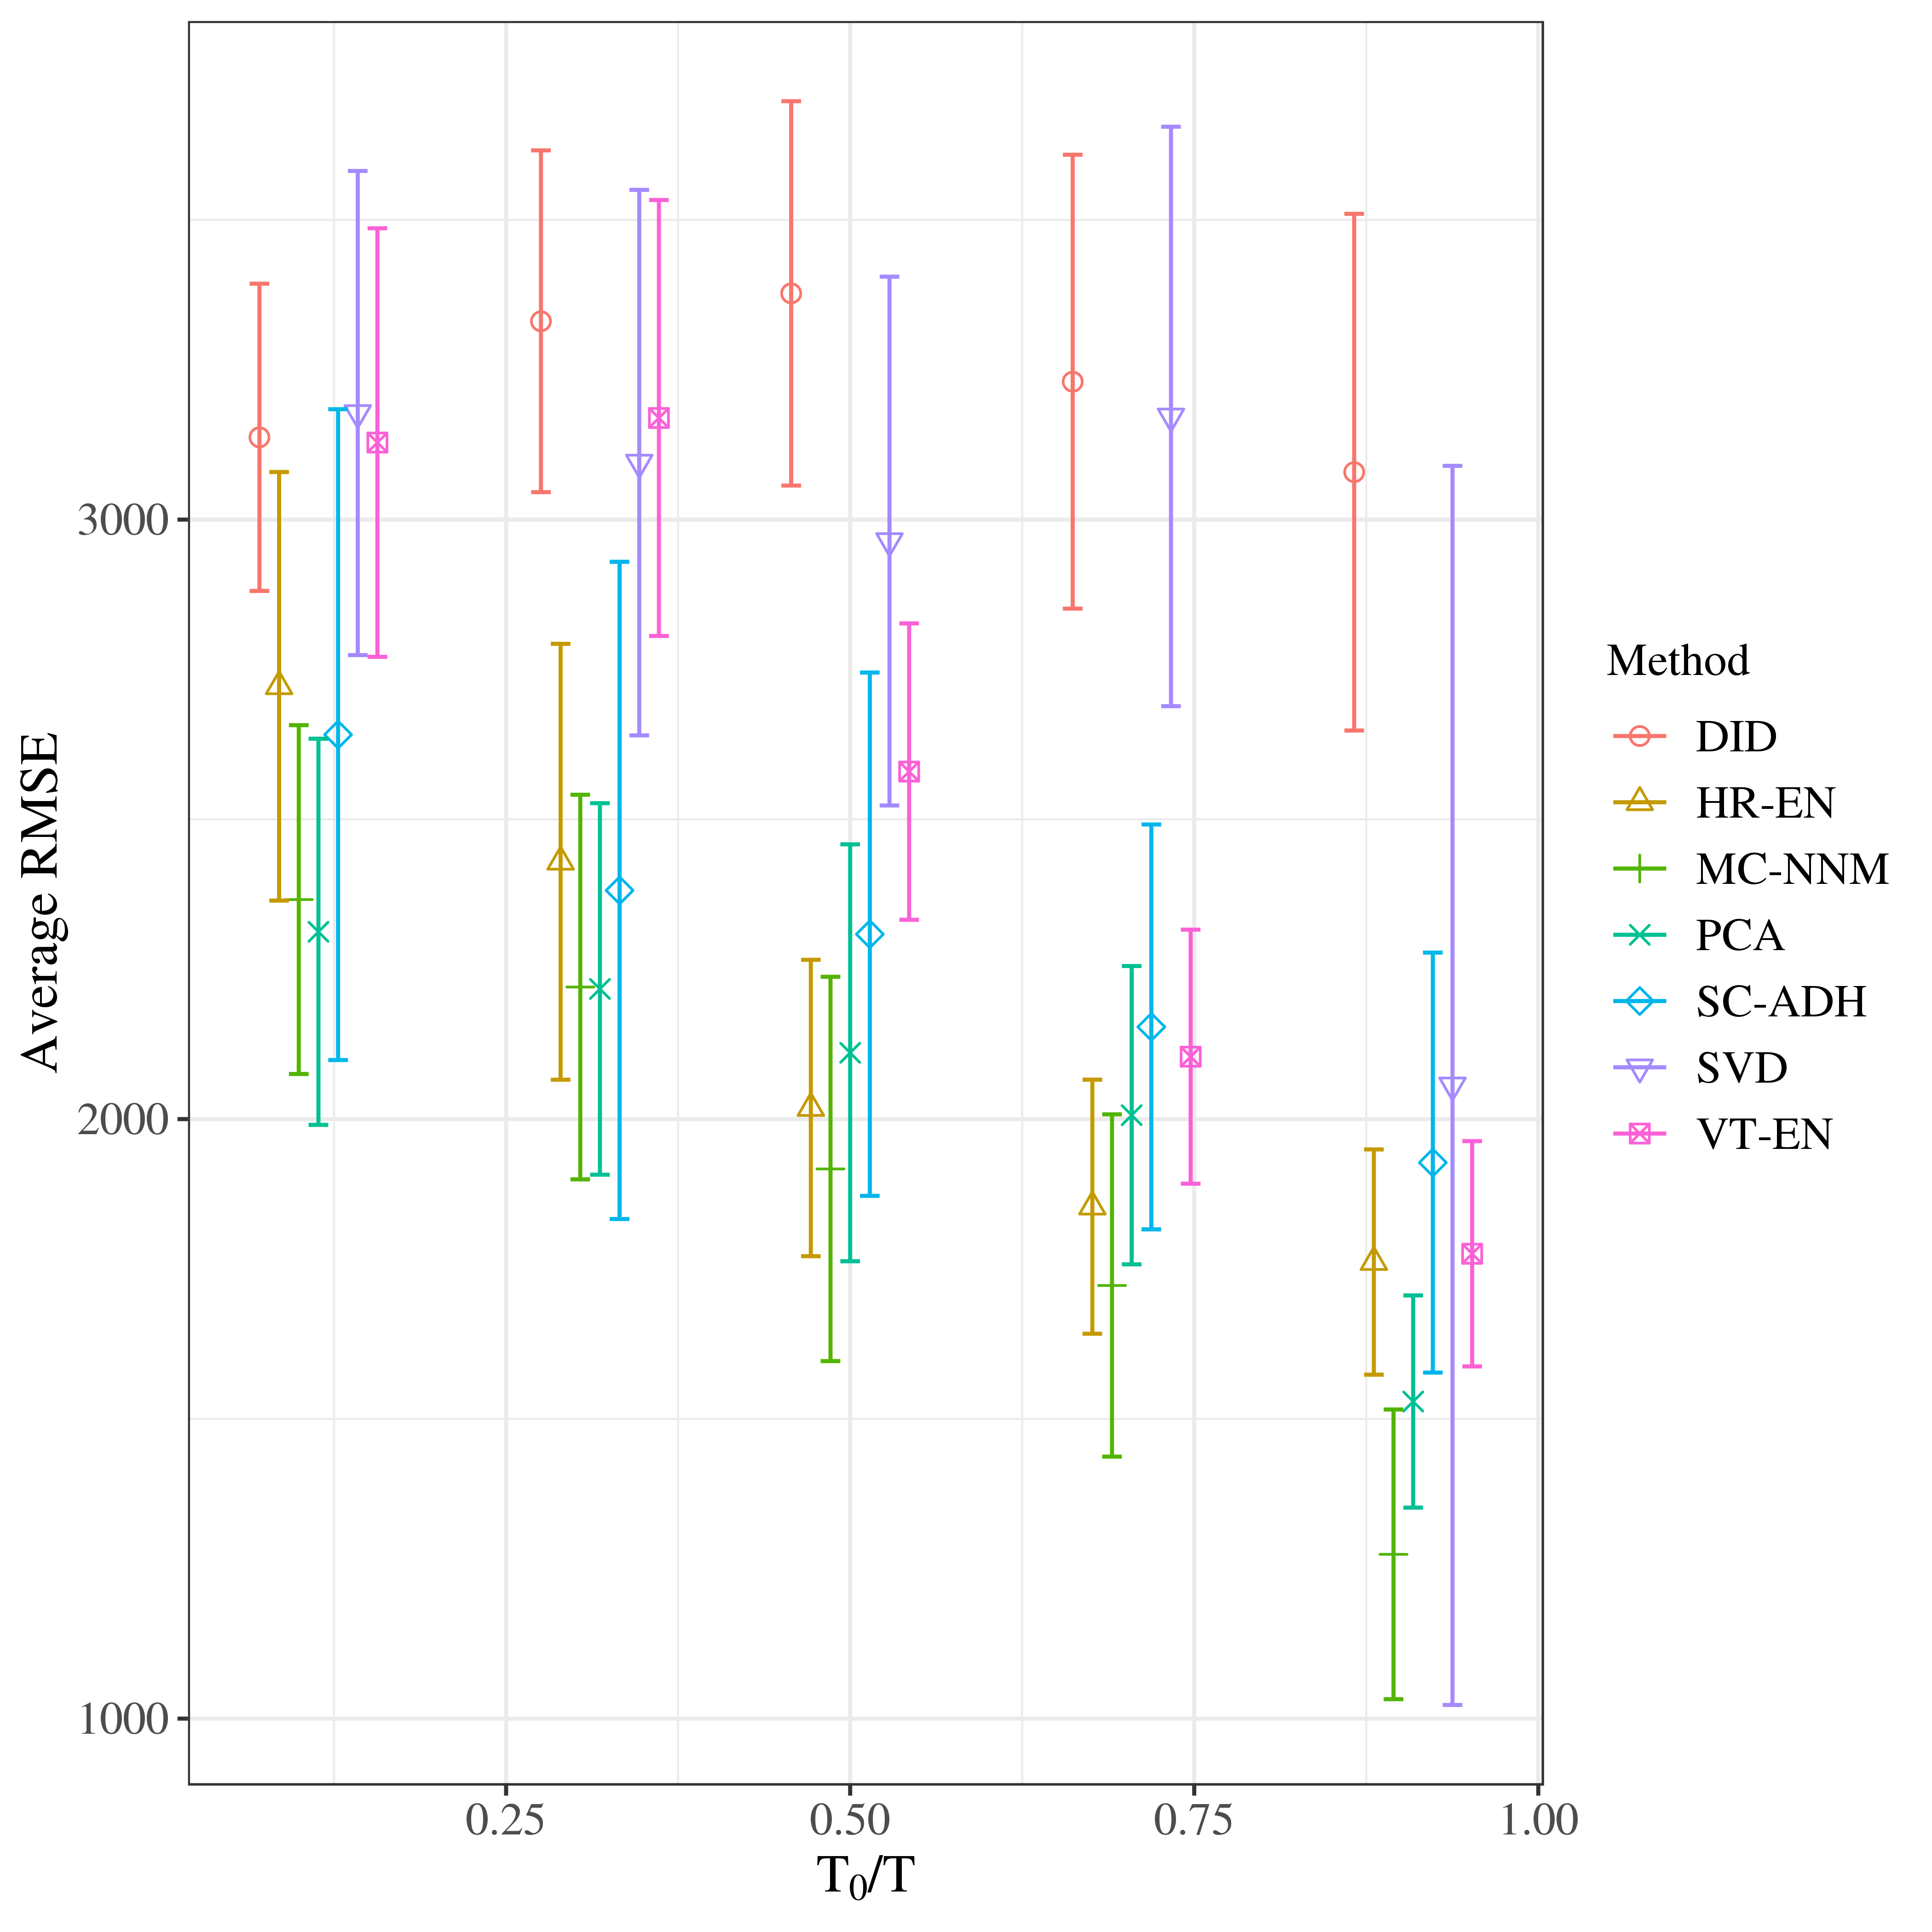
\includegraphics[width=\textwidth]{plots/germany_N_16_T_44_numruns_20_num_treated_8_simultaneuous_0.png}
		\caption{West German reunification data, $N_t = 8$}
	\end{subfigure}
	\caption{Placebo tests under staggered treatment adoption. Error bars represent 95\% confidence intervals calculated using the standard deviation of the prediction distribution for 20 trial runs. Note that the estimates are jittered horizontally to reduce overlap. \label{synth-stag}} 
\end{figure}

\subsection{Hypothesis testing} \label{hyp-test}

The method proposed by \citet{athey2017matrix} focuses estimation and does not provide guidance on hypothesis testing. Consider a setup with $J$ control units indexed by $i=1, \ldots, J$ and $Q$ treated units indexed by $i = J+1, \ldots, N$. The MC-NNM estimator imputes the missing post-period treated unit outcomes 

\[
\hat{Y}_{it} = \hat{L}_{it}, \hspace{10mm} J+1 \leq i \leq N, \, \hspace{5mm} \, T_0+1 \leq t \leq T.
\] The inferred causal effect of the intervention on the treated group is the difference between the observed outcomes of the treated units and the counterfactual outcomes that would have been observed in the absence of the intervention, 
$\hat{\alpha}_{it} = Y_{it} - \hat{Y}_{it}$ for $J+1 \leq i \leq N$ and $T_0+1 \leq t \leq T.$ Taking the difference-in-means between treated unit observed outcomes and predicted outcomes gives the per-period estimated average causal effect across treated units:

\begin{equation}
\hat{\bar{\alpha}}_{t}  = \frac{1}{Q} \sum^{N}_{i=J+1} \hat{\alpha}_{it}.  \label{eq:avg-pointwise}
\end{equation}

\noindent
\citet{chernozhukov2017exact} propose a randomization inference approach for testing the sharp null hypothesis $
\text{H}_0: \hat{\bar{\alpha}}_{t} = \bar{\alpha}^{o}_{t}$ for $T_0+1 \leq t \leq T,$
where $\left\{\bar{\alpha}^{o}_{t}\right\}_{t=T_0}^T$ is a trajectory of per-period average effects under the null. The test statistic suggested by \citet{chernozhukov2017exact} summarizes the trajectory of causal effects over the post-period:

\begin{equation} \label{tstat}
S (\hat{\bar{\alpha}}_{t}) = \left(\frac{1}{\sqrt{T_\star}} \sum_{t=T_0 +1}^{T} |\hat{\bar{\alpha}}_{t}|^q\right)^q,
\end{equation}

\noindent
where $T_\star = T-T_0$ and $q \in \left\{1, 2\right\}$. I estimate $p$-values by creating $\pi \in \Pi$ permutations of $\mathbf{Y}$ across the time dimension and calculating the proportion of test statics calculated on the permuted data under the null that are more extreme than the observed test statistic:

\begin{equation}
\hat{p} = \frac{1}{\Pi} \sum_{\pi \in \Pi} \textbf{1} \left\{S (\hat{\bar{\alpha}}_{\pi}) > S (\hat{\bar{\alpha}}_{t}) \right\}, \label{eq:pvalue}
\end{equation}

\noindent
where $\hat{\bar{\alpha}}_{\pi}$ is the average causal effect estimated on the permuted data $\mathbf{Y_\pi}$. 

The idea for permuting time periods rather than treatment assignment, as proposed by \citet{abadie2010synthetic}, is that if the data are stationary and weakly dependent, which is often the case in an aggregate time-series setting, then the distribution of the error term $\epsilon$ in (\ref{eq:mc-Y}) should be the same in the pre- and post-periods. \citet{chernozhukov2017exact} prove that the $p$-values resulting from their inferential procedure are approximately unbiased assuming that the MC-NNM estimator is consistent, which can be verified by placebo tests. 

\paragraph{Permuation structures}I rely on three types of permutations: \emph{i.i.d.} random permutations of the time index $t$; \emph{i.i.d. block} random permutations of $K=T/b$ non-overlapping blocks, where $b$ is selected according to the optimal block length for the dependent bootstrap \citep{politis2004automatic}; and \emph{moving block} permutations that circularly shift $t$ by one period, resulting in $T-1$ permutations. The latter two permutations are capable of preserving the dependence structure of the data and are thus appropriate for weakly dependent data. 

%I also construct per-period randomization confidence intervals for $\hat{\bar{\alpha}}_{t}$ via hypothesis test inversion by randomly sampling without replacement a set of null trajectories $\left\{\bar{\alpha}^{o}_{t}\right\}_{t=T_0}^T \in \mathcal{A}_t$ from a vector of evenly-spaced candidate values. For each element of $\mathcal{A}_t$, I calculate $\hat{p} (\bar{\alpha}^{o}_{t})$ using (\ref{eq:pvalue}) and return the 95\% confidence set $\mathcal{C} (t) = \bar{\alpha}^{o}_{t} \in \mathcal{A}_t: \left\{\hat{p} (\bar{\alpha}^{o}_{t}) > 0.05\right\}$. 

\section{Impact of homestead policies on state capacity} \label{state-capacity}

In this section, I estimate the causal impacts of homestead policies on state capacity, as measured by state government spending and revenue. I create measures of total expenditure and revenue collected from the records of 48 state governments during the period of 1783 to 1932 \citep{sylla1993sources} and the records of 16 state governments during the period of 1933 to 1937 \citep{sylla1995sourcesa,sylla1995sourcesb}. Comparable measures for 48 states are drawn from U.S. Census special reports for the years 1902, 1913, 1932, 1942, 1962, 1972, and 1982 \citep{haines2010}.\footnote{I take the mean of duplicate state-year observations, which arise for the years 1902, 1913, and 1932.} The expenditure measure includes state government spending on education, social welfare programs, and transportation. The revenue measure incorporates state government income streams such as tax revenue and non-tax revenues such as land sales.\footnote{Tax revenue is commonly used as a measure of fiscal capacity \citep{lieberman2002taxation}, which is the bureaucratic ability of governments to raise taxes from multiple sources in order to finance policies. Fiscal capacity is strongly correlated with state capacity \citep{besley2010state}.} 

The data pre-processing steps are as follows. Each measure is inflation-adjusted according to the U.S. Consumer Price Index \citep{williamson2017seven} and scaled by the total free population in the decennial census \citep{haines2010}. Missing values are imputed separately in the pre- and -post-periods by carrying the last observation forward and remaining missing values are imputed by carrying the next observation backward. The raw outcomes data are log-transformed to alleviate exponential effects. Lastly, I remove states with no variance in the pre-intervention outcomes results in complete $N \times T$ matrices of size $33 \times 159$ and $34 \times 158$, for the expenditures and revenues outcomes, respectively. 

The staggered adoption setting is appropriate for the current application because the year of initial treatment exposure $T_0$ varies across states, about half of which are exposed to homesteads following the passage of the HSA. I determine the years of initial exposure to homesteads by aggregating to the state level approximately 1.46 million individual land patent records authorized under the HSA.\footnote{Land patent records provide information on the initial transfer of land titles from the federal government and are made accessible online by the U.S. General Land Office (\url{https://glorecords.blm.gov}).} The earliest homestead entries occurred in 1869 in about half of the western frontier states, about seven years following the enactment of the HSA. In 1872, the first homesteads were filed in southern PLS.\footnote{Figure SM-\ref{fig:homestead-heatmap} visualizes the timing and intensity of homestead entries.} 

When estimating (\ref{eq:mc-Y}), unit-specific covariates $\mathbf{X}$ include state-level average farm sizes measured in the 1860 and average farm values measured in the 1850 and 1860 censuses. In theory, we should expect that homesteaders migrate to more productive land and thus excluding these pre-intervention measures of agricultural productivity may result in overestimating the actual impact of homestead policies. To control for selection bias arising from differences in access to frontier lands, I create a measure of railroad access using digitized railroad maps provided by \citet{atack2013use}, which contain information on the year that each rail line was built. Overlaying the railroad track map over historical county borders, I calculate the total miles of operational track per square mile and aggregate the measure to the state-level.\footnote{Using these data, I estimate that 29\% of counties had railroad access in 1862 and 91\% had access by 1911 (Fig. SM-\ref{rr-map}). The railroad access measure defines access with respect to county boundaries, which \citet{atack2012impact} point out has limitations because a county without access might be adjacent to one with access and county boundaries frequently changed over time.}

\subsection{Placebo tests} \label{placebo-tests}

Prior to presenting the main results, I assess the validity of the key assumption underlying the approach by discarding post-period observations from the data and testing the null hypothesis 

\begin{equation} \label{h0-placebo}
\text{H}_0: S (\hat{\bar{\alpha}}_{t}) = 0  \, \hspace{5mm} \,  \text{for} \, \hspace{2mm} T_0 - \tau +1 \leq t \leq T_0,
\end{equation}
%\frac{1}{\tau +1} \sum_{T_0 - \tau +1}^{T_0} \hat{\bar{\alpha}}_{t} 
\noindent
where $\tau \in \left\{1, 10, 25\right\}$. This placebo null hypothesis is tested by the same procedure described in Section \ref{hyp-test}, treating $\left\{1, \ldots, T_0 - \tau\right\}$ as the pre-period.

Table \ref{placebo-tests} reports the average treatment effect over the placebo post-period and randomization $p$-values calculated by (\ref{eq:pvalue}). Placebo tests on the revenue outcome yield two-sided $p$-values greater than the significance level of $\alpha = 0.05$, regardless of the value of $q$ or permutation structure. These results provide evidence in favor of the validity of the consistency assumption. However, we can only reject the null in the case of $\tau=1$ when considering the expenditure outcome. 

\begin{table}[htbp]
	\captionsetup{font=normalsize}
	\caption{Placebo test $p$-values.\label{placebo-tests}}
	\begin{center}
		\scalebox{.95}{\begin{tabular}{@{}lccccccccc@{}}
		\toprule
		 & \multicolumn{3}{c}{Education Spending}        & \multicolumn{3}{c}{Expenditure}            & \multicolumn{3}{c}{Revenue}                \\ \midrule
		& $\tau = 10$   & $\tau = 20$   & $\tau = 30$   & $\tau = 10$  & $\tau = 20$  & $\tau = 30$  & $\tau = 10$  & $\tau = 20$  & $\tau = 30$  \\
		\hline
		Mean Effect                          & -0.43         & -0.34         & -0.26         & 0.1          & 0.05         & 0.02         & 0.05         & 0.03         & 0.03         \\
		i.i.d. Block CIs                       & [-1.45, 1.45] & [-1.07, 1.11] & [-0.62, 0.67] & [0.00, 0.00] & [0.00, 0.00] & [0.00, 0.00] & [0.00, 0.00] & [0.00, 0.00] & [0.00, 0.00] \\
		Moving Block CIs                       & [-1.16, 1.23] & [-0.95, 0.92] & [-0.62, 0.69] & [0.00, 0.00] & [0.00, 0.00] & [0.00, 0.00] & [0.00, 0.00] & [0.00, 0.00] & [0.00, 0.00] \\ \bottomrule
\end{tabular}
}
	\end{center}
	\footnotesize{\emph{Notes:} randomization $p$-values corresponding to each permutation structure and value of $\tau$ and $q$. i.i.d. block and i.i.d. block $p$-values are calculated using $|\Pi| = 1,000$ permutations. Moving block $p$-values are based on $|\Pi| = T-1$ permutations.}
\end{table}

Further evidence of the consistency of the MC-NNM estimator is provided in Figure SM-\ref{mc-sim}, which presents the results of placebo tests on control units using both pre- and post-period observations. Similar to the simulations on the synthetic control datasets discussed in Section \ref{sims}, there are no missing entries in each outcome $\mathbf{Y}$ because the actual treated units are removed prior to the placebo tests. I randomly choose about half of the remaining control units as hypothetical treated units and predict their values for time periods following a randomly selected $T_0$. The MC-NNM estimator outperforms DID and SVD estimators in terms of minimizing RMSE for each ratio $T_0/T$. At $T_0/T \geq 0.5$, the estimator generally yields comparable error rates to PCA, synthetic control, and vertical regression estimators. 

\subsection{Main estimates} \label{main-estimates}

In the main analyses, I fit the MC-NNM estimator described in (\ref{eq:mc-Y}) on the entirety of observed entries in $\mathbf{Y}$ to recover its missing entries; i.e., the counterfactual outcomes of PLS. The value of the regularization term $\lambda$ is optimally selected on the value that yields the lowest average RMSE calculated during cross-validation. The average RMSE calculated on the validation sets during the $\lambda$ selection process are 0.41 and 0.48 for the expenditures and revenues outcomes, respectively. 

The top panels of Figure \ref{mc-estimates-exp-pc} and \ref{mc-estimates-rev-pc} compare the observed time-series of treated units and control units along with the predicted outcomes of treated units. The observed means of the treated and control units are essentially identical in the post-period. However, we are interested primarily in the difference in the observed and predicted treated unit outcomes, which is the quantity $\hat{\bar{\alpha}}_{t}$, which corresponds to the estimated per-period average causal effects of treatment exposure on the treated units. These per-period causal impacts are plotted in the bottom panels. Bootstrap confidence intervals for $\hat{\bar{\alpha}}_{t}$ are calculated by block resampling with optimal block lengths selected by the procedure described by \citet{politis2004automatic}. 

The per-period impact time-series for both outcomes are essentially zero during the pre-period and within the bounds of the bootstrap confidence intervals, which demonstrates that the model is closely fitting the pre-period observations. Per-period impacts on state government spending peak in 1870, at the same time most PLS were first exposed to homesteads, representing a 0.18 [-0.35, 0.71] log increase in per-capita expenditure. By 1876, after most PLS had been exposed to homesteads, homestead exposure decreases expenditure by 0.51 [-1.67, 0.66] log points, and the trajectory of causal impacts remains negative for the rest of the time-series. Similarly, per-period impacts on revenue peak in 1873, representing a 0.43 [-0.57, 1.44] log increase in per-capita revenues, at the same time southern PLS are exposed to homesteads. The causal impacts on revenue quickly decrease and remain negative for the remaining time-series; in 1877, exposure to homesteads confer a 0.45 [-1.51, 0.61] log point decrease in per-capita revenue. 

\begin{figure}[htbp]
	\centering
%	\begin{subfigure}[t]{0.48\textwidth}
%		\centering
%		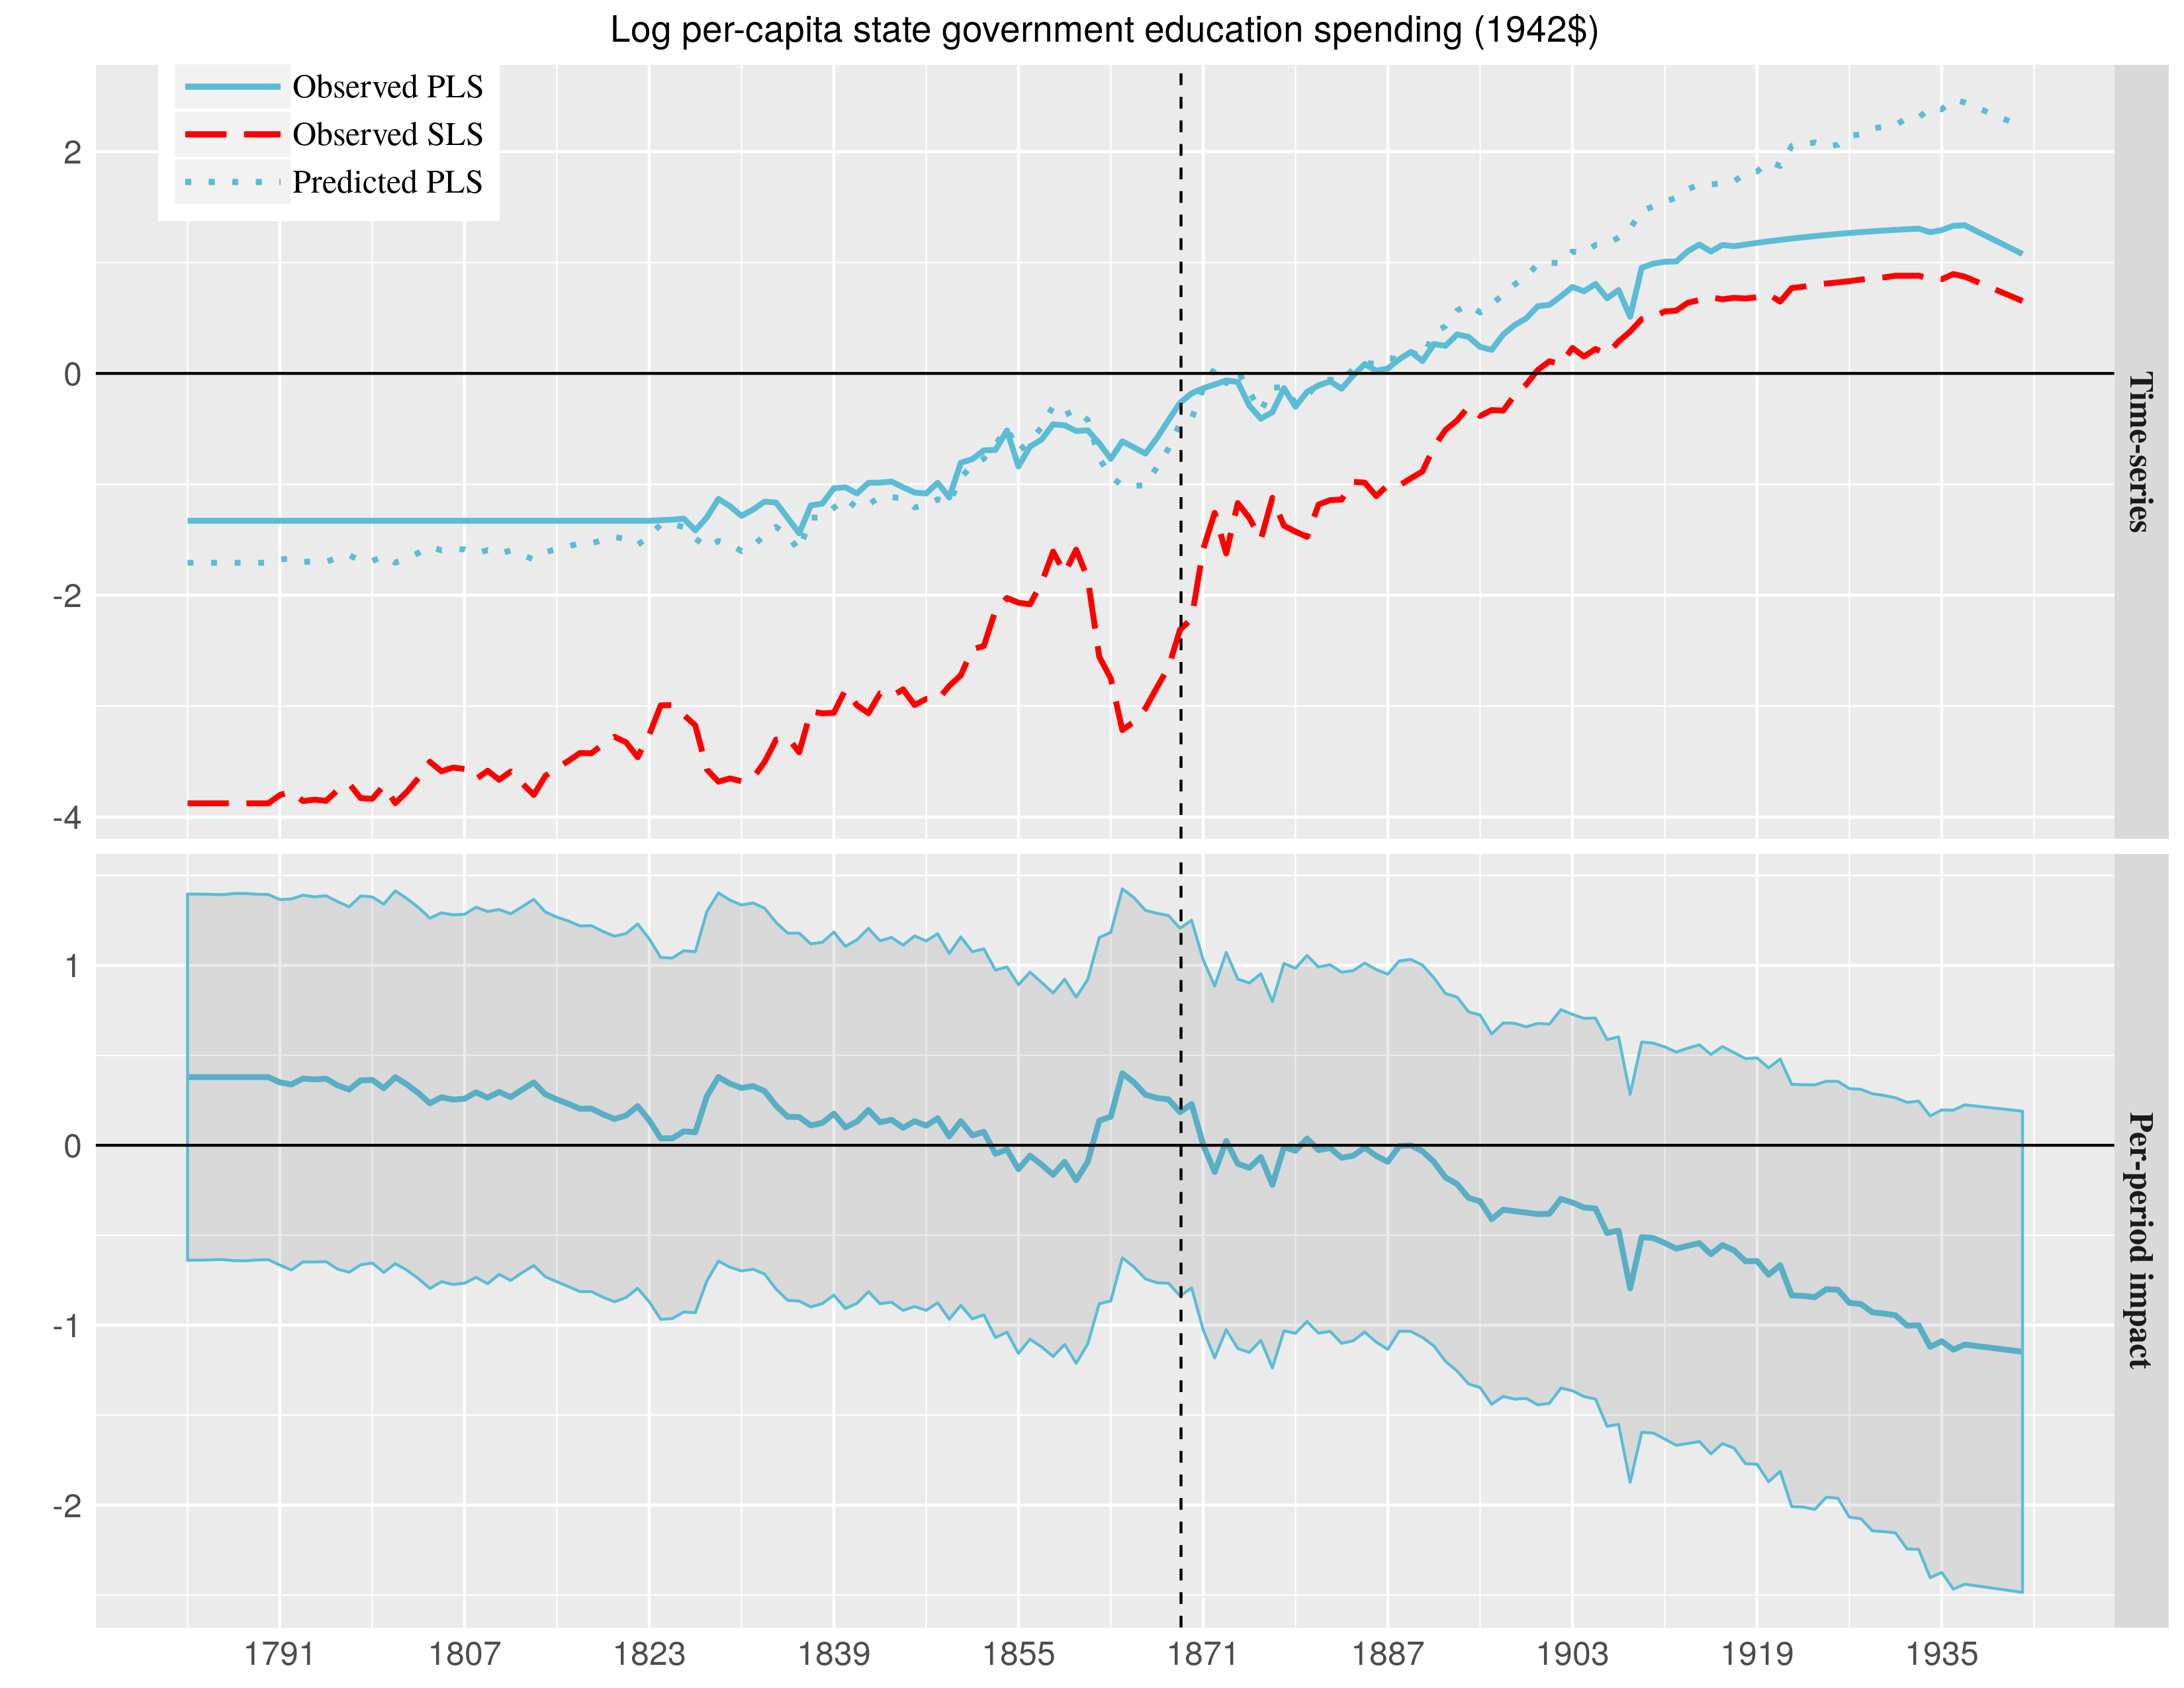
\includegraphics[width=\textwidth]{plots/mc-educ-pc.png}
%		\caption{State government education spending}
%	\end{subfigure}
%	~ 
	\begin{subfigure}[t]{0.75\textwidth}
		\centering
		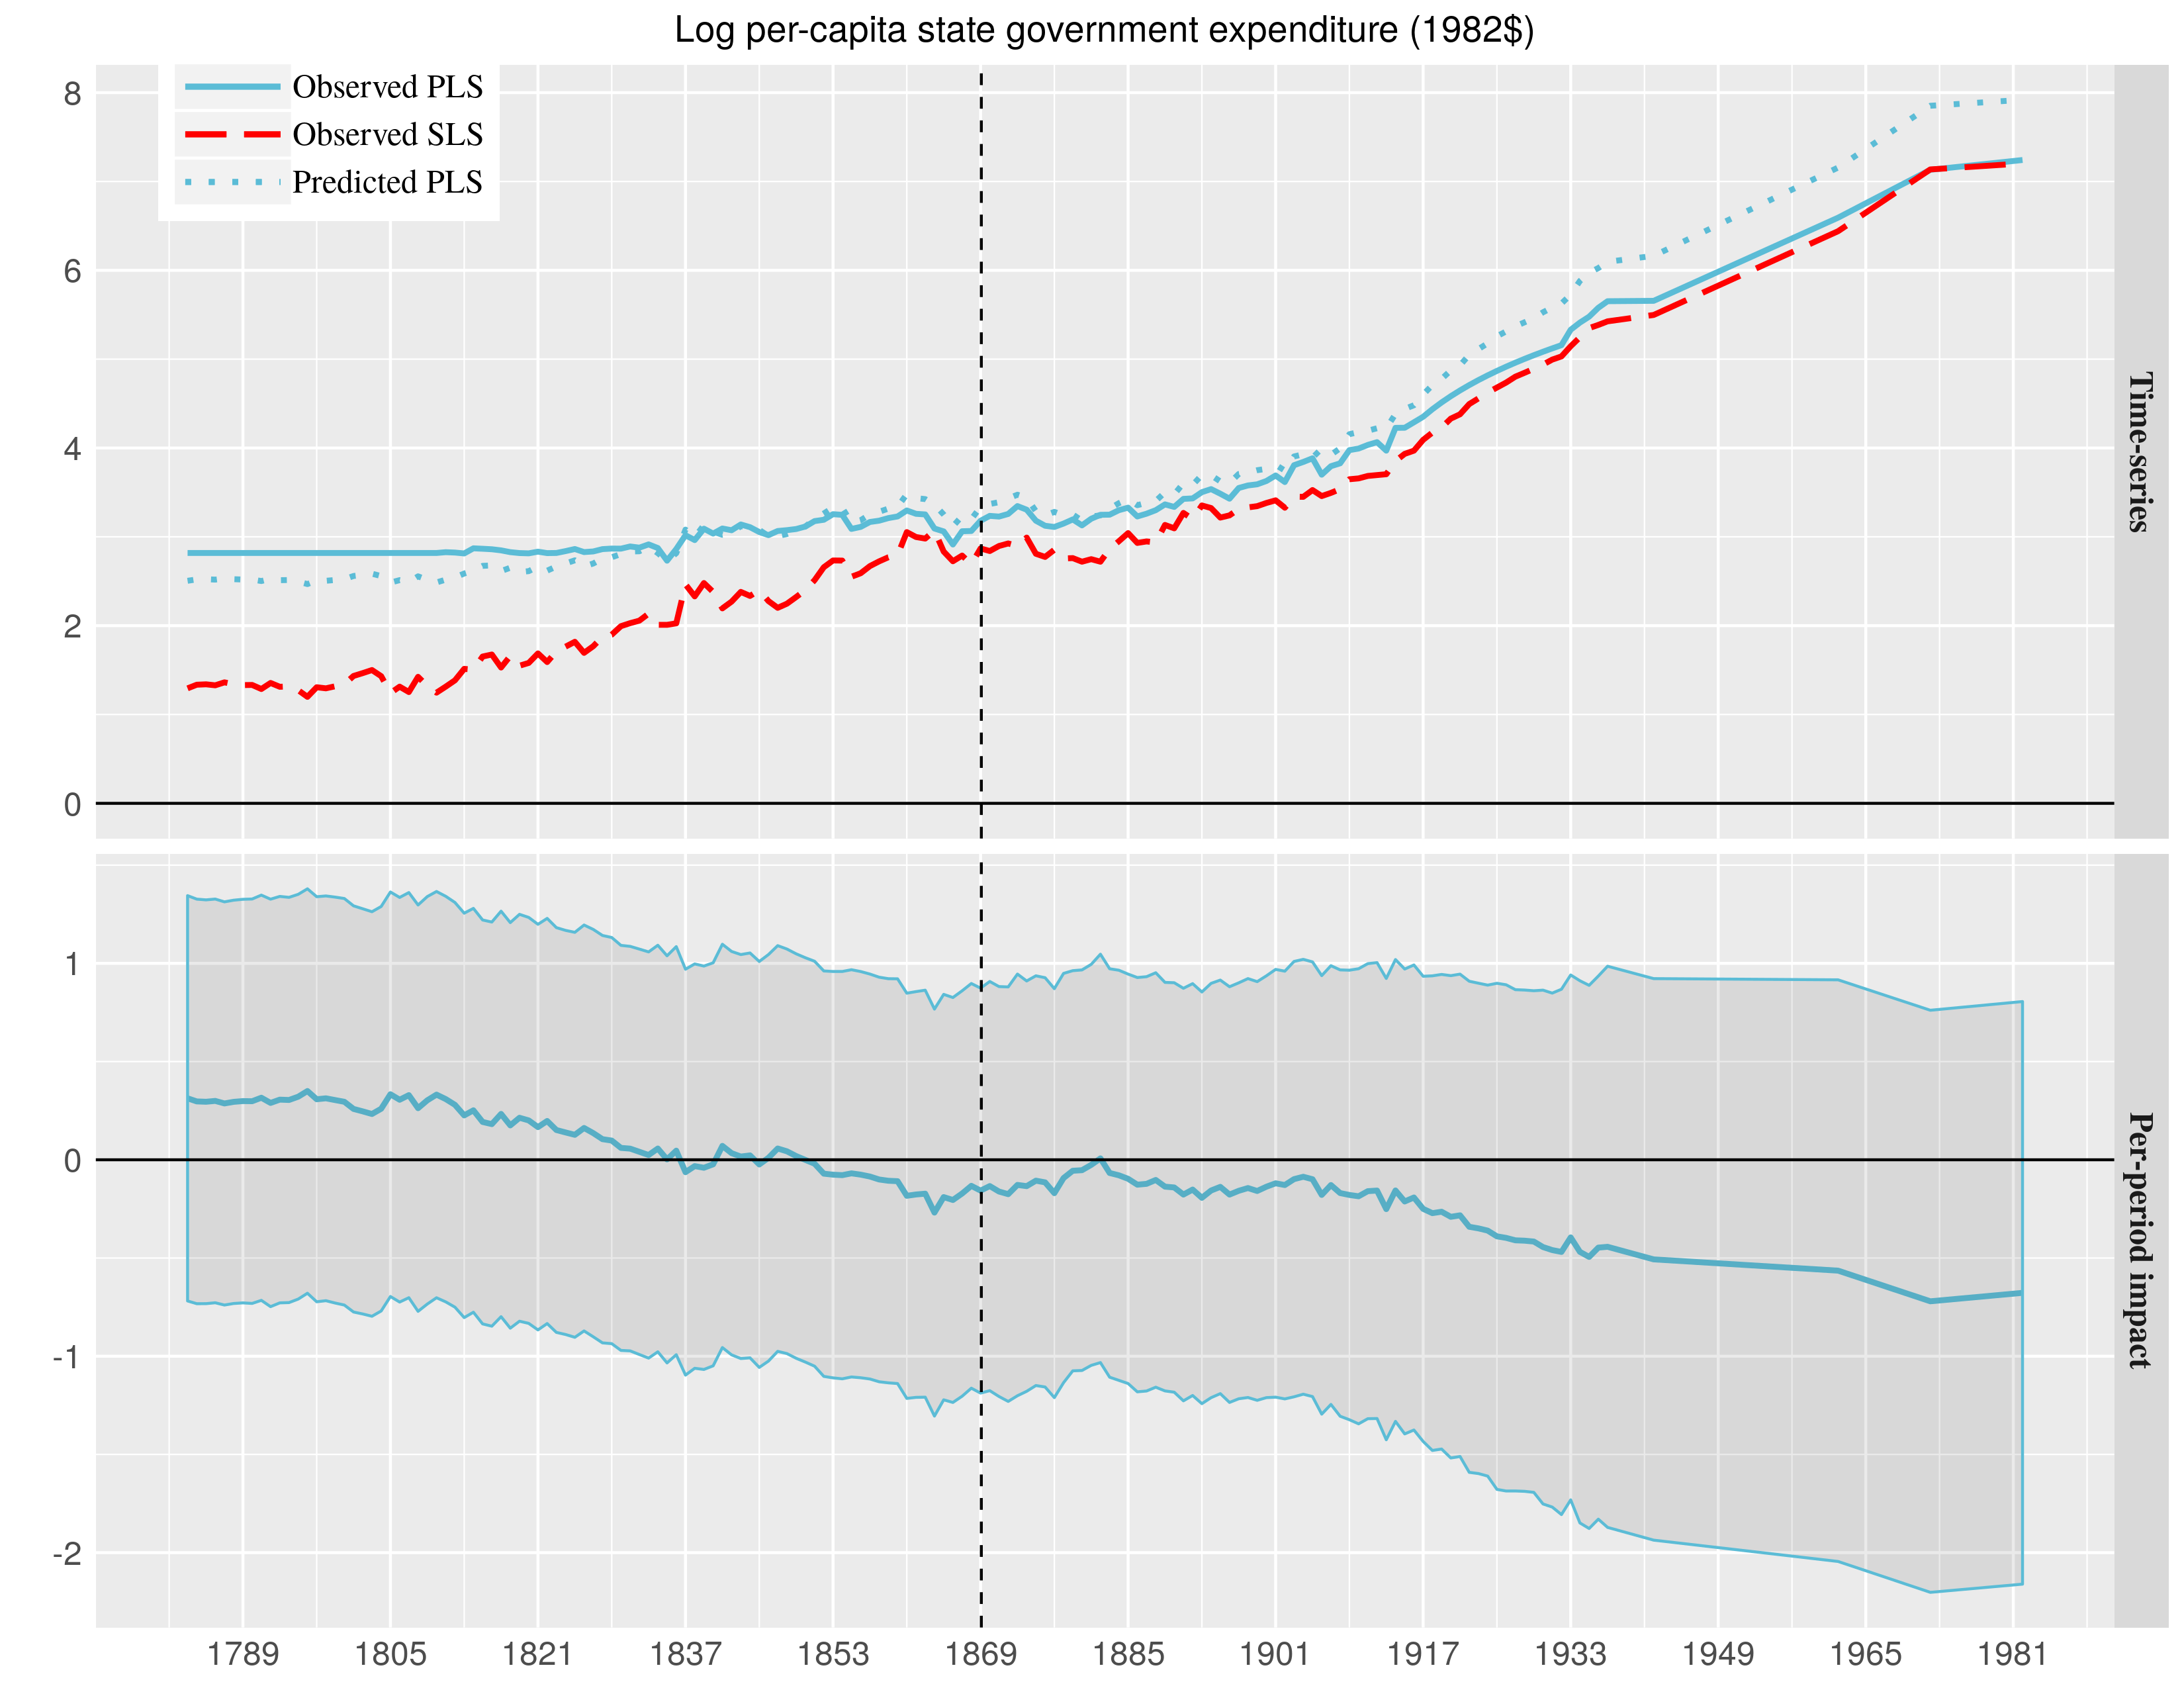
\includegraphics[width=\textwidth]{plots/mc-exp-pc.png}
		\caption{Log per-capita state government expenditure (1982\$)\label{mc-estimates-exp-pc}}
	\end{subfigure}
	~ 
	\begin{subfigure}[t]{0.75\textwidth}
		\centering
		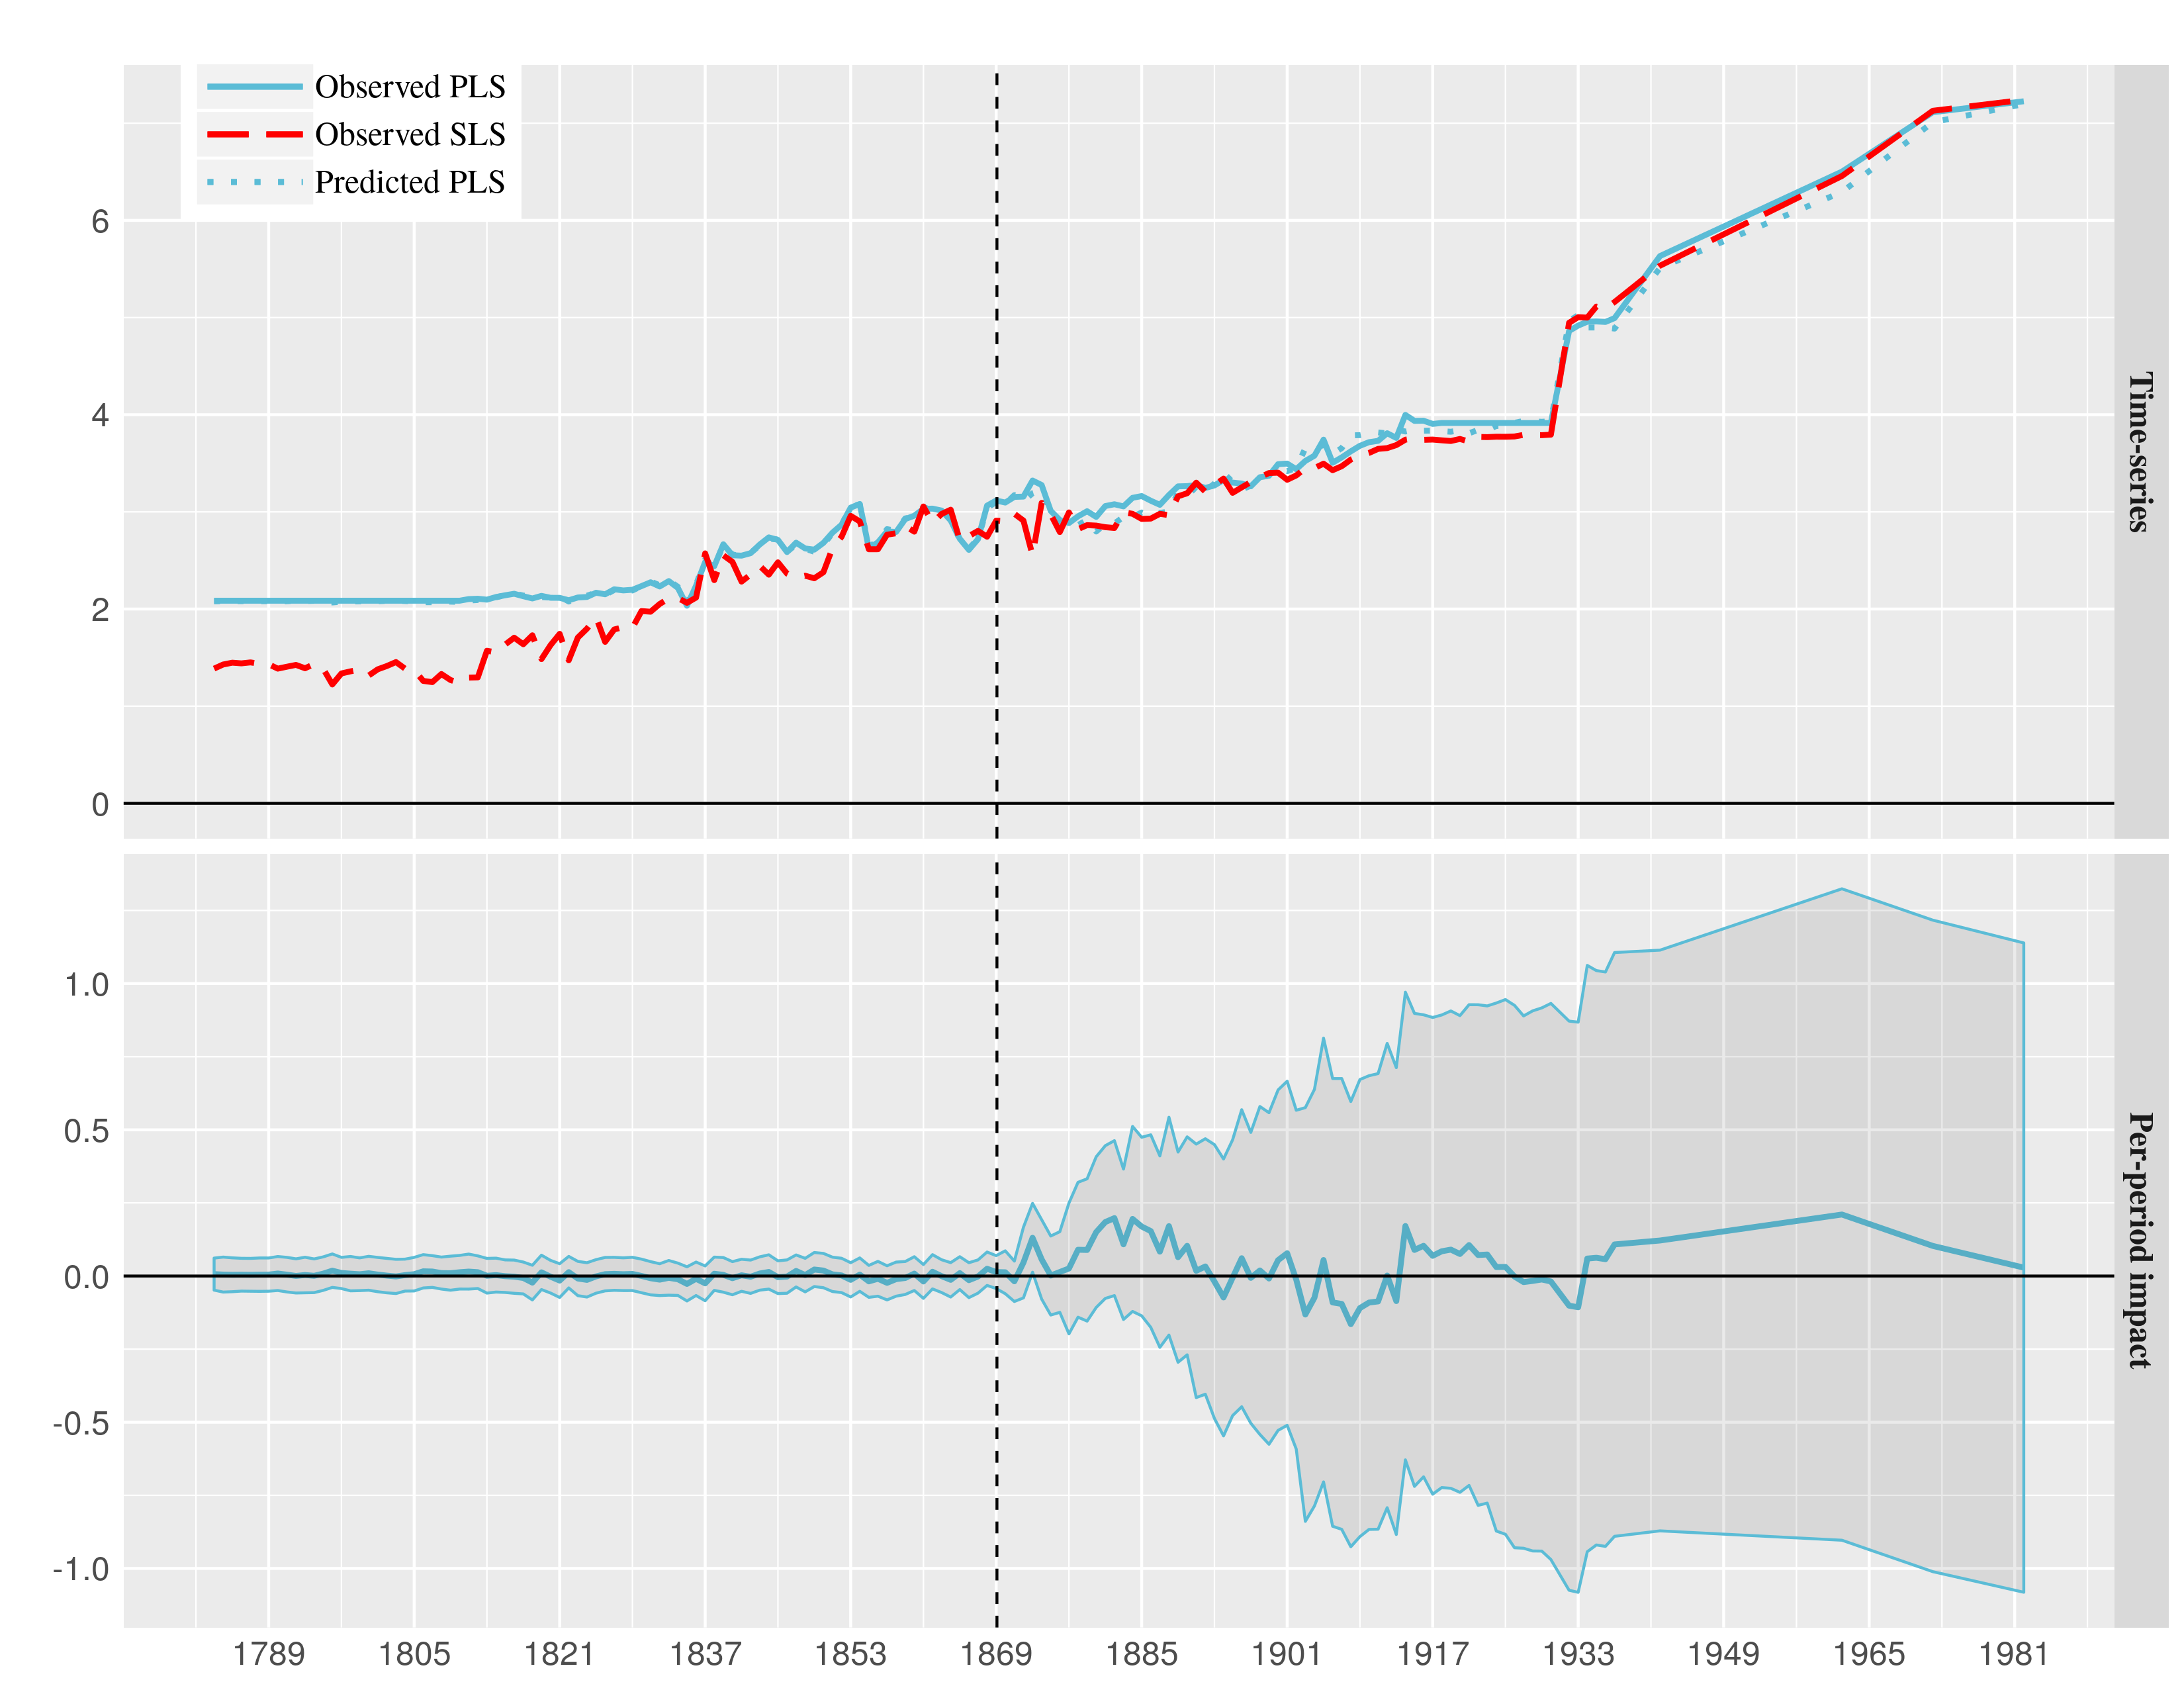
\includegraphics[width=\textwidth]{plots/mc-rev-pc.png}
		\caption{Log per-capita state government revenue (1982\$)\label{mc-estimates-rev-pc}}
	\end{subfigure}
	\caption{Top panel: Mean observed (solid time-series) and counterfactual predicted (dotted time-series) outcomes of treated units (PLS) and mean observed outcomes (dashed time-series) among control units (SLS), displayed for the time period of 1809 to 1982. Dashed vertical line represents the initial treatment year of 1869. Bottom panel: Per-period average causal impacts of homestead exposure on PLS, or $\hat{\bar{\alpha}}_{t}$ in (\ref{eq:avg-pointwise}). Shaded regions represent 95\% confidence intervals estimated by taking $\hat{\bar{\alpha}}_{t} \pm 1.96$ the standard error of the distribution of 1,000 bootstrap replicates of $\hat{\bar{\alpha}}_{t}$.\label{mc-estimates}} 
\end{figure}

The estimated bootstrap confidence intervals are useful for evaluating per-period causal impacts but are not helpful in evaluating the overall effect of homestead policies. Table \ref{mc-estimates} reports randomization $p$-values from testing the null hypothesis of a zero effect:

\begin{equation} \label{h0}
\text{H}_0: S (\hat{\bar{\alpha}}_{t}) = 0  \, \hspace{5mm} \,  \text{for} \, \hspace{2mm} T_0 + 1 \leq t \leq T.
\end{equation}
\noindent

The null hypothesis (\ref{h0}) can rejected at the 5\% level for both outcomes, both values of $q$, and all three permutation schemes. Note that the relevant test statistic $S (\hat{\bar{\alpha}}_{t})$ measures the trajectory of average causal effects in absolute terms and thus does not provide information on the direction or evolution of the causal effects over time. %Figures 9 and 10 display pointwise 90\% confidence intervals. We find similar results for all three methods, which suggest that, while the effect was not or only marginally significant in the first year, legalizing indoor prostitution significantly decreased both rape rates and the incidence of female gonorrhea thereafter.

\begin{table}[htbp]
	\captionsetup{font=normalsize}
	\caption{Testing the null hypothesis (\ref{h0}).\label{mc-estimates}}
	\begin{center}
		%\begin{tabular}{@{}lcc@{}}
%	\toprule 
%	& \multicolumn{2}{c}{ Education Spending } \\
%\hline
%	& $q=1$ & $q=2$ \\
%\hline \\
%	$S (\hat{\bar{\alpha}}_{t})$ & 3.81 & 1.66 \vspace{2mm}\\
%	i.i.d. & 0 & 0 \\
%	i.i.d. Block & 0.02 & $<0.01$3 \\
%	Moving Block & 0.23 & 0 \\
%		 &  &  \\
%	& \multicolumn{2}{c}{ Expenditure }\\
%\hline
%	& $q=1$ & $q=2$ \\
%\hline \\
%	$S (\hat{\bar{\alpha}}_{t})$ & 1.99 & 0.81\vspace{2mm} \\
%	i.i.d. & 0.39 & 0.49 \\
%	i.i.d. Block & 0.50 & 0.49 \\
%	Moving Block & 0.41 & 0.38 \\
%			 &  &  \\
%	& \multicolumn{2}{c}{ Revenue }\\
%\hline
%	& $q=1$ & $q=2$ \\
%\hline \\
%	$S (\hat{\bar{\alpha}}_{t})$ & 1.28 & 0.62\vspace{2mm} \\
%	i.i.d. & 0.99 & 0.85 \\
%	i.i.d. Block & 0.89 & 0.64 \\
%	Moving Block & 0.74 & 0.41 \\
%\bottomrule
%\end{tabular}
\begin{tabular}{@{}lcccc@{}}
	\toprule 
	& \multicolumn{2}{c}{ Expenditure } & \multicolumn{2}{c}{ Revenue } \\
	\hline
	& $q=1$ & $q=2$ & $q=1$ & $q=2$ \\
	\hline \\
	$\text{S}_q (\boldsymbol{\hat{\bar{\upalpha}}})$ & 3.87 & 1.40 & 1.97 & 0.76\vspace{2mm}\\
	i.i.d. & 0.002 & 0.003 & 0.001 & 0.001\\
	i.i.d. Block & 0.001 & 0.002 & 0.001 & 0.001\\
	Moving Block & $<0.001$ & $<0.001$ & $<0.001$ & $<0.001$ \\
	\bottomrule
\end{tabular}

	\end{center}
	\footnotesize{\emph{Notes:} $S (\hat{\bar{\alpha}}_{t})$ corresponds to the test statistic described in (\ref{tstat}) and each value beneath is the randomization $p$-value corresponding to each permutation structure. See footnotes to Table \ref{placebo-tests}.}
\end{table}

\section{DID estimation} \label{DID}

The matrix completion approach estimates the impact of a binary exposure to treatment on a continuous outcome. However, in this application a continuous form of treatment is available in the form of homestead entries. Equation (\ref{eq:dd}) estimates a continuous version of the DID estimator described in Section \ref{sims}, where the first difference comes from variation in the date of initial exposure to homesteads, and the second difference comes from variation in the intensity of homestead entries:

\begin{equation} 
Y_{it} =  \gamma_i + \delta_t + \psi \, M_{it} + \phi \, (M_{it} \cdot \text{homesteads}_{it}) + X_{it}  + \epsilon_{it}. \label{eq:dd} 
\end{equation}

\noindent
$\gamma_i$ and $\delta_t$ are state and year effects, respectively, and $X_{it}$ is a matrix of unit- and time-varying covariates included to control for parallel trends in agricultural productivity and access to frontier lands. In the staggered adoption setting, entries in the treatment indicator $M_{it} = 1$ at $t \geq T_0$, where the initial exposure time $T_0$ varies across units. The continuous treatment exposure variable $\text{homesteads}_{it}$ measures the per-capita statewide sum of homestead entries in state $i$ and year $t$.

The coefficient corresponding to the interaction term, $\hat{\phi}$, is the estimated average causal effect of exposure to homesteads. I use unit-stratified bootstrapped samples to construct nonparametric standard errors for $\hat{\phi}$.\footnote{The model assumes i.i.d. errors, which understates the standard errors for $\hat{\delta}$ when the regression errors are serially correlated, or $\mathrm{Corr} (\epsilon_{it}, \epsilon_{i,t-1}) \neq 0$, which can arise when the time-series lengths are not sufficiently long to reliably estimate the data generating process. \citet{bertrand2004much} show that the stratified bootstrap can be used to compute consistent standard errors when the number of units is sufficiently large.} 

Similar to the case of binary treatment, the continuous DID estimator is adapted to a setting of staggered adoption because the initial date of exposure to homesteads varies across PLS. It should be emphasized that estimating (\ref{eq:dd}) in a staggered adoption setting relies on several strong assumptions regarding both the assignment mechanism, which in this application is the distribution of initial treatment times $T_0$, and the counterfactual outcomes of the treated units. The framework of \citet{athey2018design}, for instance, assumes the distribution of $T_0$ is completely random conditional on the covariates. In the current application, this assumption ignores the possibility that initial exposure to homesteads might be determined by unobserved factors. The framework also that the counterfactual outcomes at time $t$ does not depend on the future date of treatment exposure if $t < T_0$ or the history of treatment exposure if $t > T_0$. Violations of these assumptions would arise if the homestead policies is anticipated prior to $T_0$ or if the size of frontier state government is determined by whether the state was exposed early or late to homesteads. 

\subsection{DID estimates on state capacity}

I estimate (\ref{eq:dd}) on balanced state-year panel datasets covering state government finances from the years 1783 to 1982. The covariate matrix $X_{it}$ includes measures of railroad access, farm sizes, and farm values. Missing values in $X_{it}$ are imputed separately in the time periods before and after 1868, carrying the last observation forward and impute remaining missing values by carrying the next observation backward. 

Table \ref{dd-estimates} reports the treatment effect estimates corresponding to the interaction term $\hat{\phi}$. The estimates indicate that a 10\% increase in log per-capita homesteads is expected to significantly decrease log per-capita stage government finances by about 0.1\%. The point estimates are considerably smaller in magnitude -- albeit in the the same direction-- as the per-period MC-NNM estimates presented in Section \ref{main-estimates}. The bootstrap confidence intervals around the DID estimates are considerably more narrow than those for the MC-NNM per-period impacts displayed in Figure \ref{mc-estimates} and most likely overoptimistic due to serial correlation in the DID regression errors.

\begin{table}[htbp]
	\begin{center}
		\caption{DID estimates: Impact of homestead entries on per-capita state government finances and land inequality. \label{dd-estimates}}
		\resizebox{.8\width}{!}{	\begin{tabular}{@{}lccc@{}}
		\toprule
		& Expenditure             & Revenue                 & Land inequality \\ \midrule
		Treatment effect ($\hat{\phi}$) & -0.013  &  -0.012  &   -4.81 $\cdot\,10^{-4}$        \\
										 &  [-0.018, -0.009] &  [-0.017, -0.008] &   [-9.756 $\cdot\,10^{-4}$, -4.636 $\cdot\,10^{-5}$]         \\
									  &                   &                    &          \\
		Adjusted $R^2$                           & 0.74                    & 0.73                    &   0.84         \\
		$N$                             & 5,247                   & 5,372                  &  463          \\
		Includes farm size \& railroad access                      & Yes                  & Yes                 &  No         \\
		Includes farm values                      & Yes                  & Yes                 &  Yes         \\
		Includes state \& year effects               & Yes                  & Yes                 &  Yes         \\
		 \bottomrule
	\end{tabular}
}
	\end{center}
	\footnotesize{Notes: Values in brackets represent 95\% confidence intervals constructed using 1,000 state-stratified bootstrap samples.}
\end{table}

\subsection{Land inequality as a causal mechanism}  \label{mechanisms}

Through which channels do homesteads affect state capacity? The political economy literature is largely in agreement that inequality and state capacity are inversely related. The canonical model of \citet{meltzer1981rational} predicts a positive relationship between inequality and redistribution because greater inequality implies the median voter is poorer than the average voter, which in turn increases demand for redistribution in majority-rule elections. However, models that allow for differences in political influence across economic groups predict an inverse relationship. In \possessivecite{benabou2000unequal} model, the pivotal voter is wealthier than the median and has the power to block redistribution as inequality increases. In \possessivecite{besley2009origins} framework, greater economic power of the ruling class reduces investment in state capacity. 

Landed elites might choose an inefficient organization of the state in order to create inefficiencies in tax collection \citep{acemoglu2011emergence} or ``hollow-out'' tax institutions in order to constrain the state's ability to tax in the future \citep{suryanarayan2017hollowing}. Similarly, \citet{galor2009inequality} propose a model where wealthy landowners block education reforms because education favors industrial labor productivity and decreases the value in farm rents. Inequality in this context can be thought of as a proxy for the amount of \emph{de facto} political influence elites have to block reforms and limit the capacity of the state \citep{acemoglu2008persistence}. 

To test whether homesteads affected future land inequality in frontier counties, I calculate a commonly-used measure of land inequality based on the Gini coefficient of census farm sizes. Gini-based land inequality measures are commonly used as proxy for the \emph{de facto} bargaining power of landed elites \citep[e.g.,][]{boix2003democracy,ziblatt2008does,ansell2015}. Note that the Gini coefficient will underestimate land inequality in counties with high shares of propertyless farmers because tenant farms are included in the farm size data, which is problematic because farms can be operated by different tenants but owned by the same landlord. I correct for this problem by adjusting the farm Gini coefficient $G$ by the ratio of farms to adult males, $p$, as recommended by \citet{vollrath2013inequality}.\footnote{The adjusted coefficient is calculated as $G^A = p G + (1-p)$.} 

In Figure SM-\ref{fig:ineq-capacity}, a bivariate regression model yields a positive relationship between land inequality and state government finances during the period of 1860 to 1950, especially at higher levels of inequality. This relationship points to inequality as a potential causal mechanism underlying the relationship between homesteads and state capacity.\footnote{However, this relationship is subject to reverse causality because state policies determining expenditures and revenue can also shape the distribution of landownership.} The inverse relationship is consistent with the findings of \citet{ramcharan2010inequality} and \citet{vollrath2013inequality} in the context of taxes, revenues, and public school spending at the county-level in 1890 and 1930.

Table \ref{dd-estimates} presents DID estimates of the impact of log per-capita homesteads on land inequality at the state-level during the period of 1870 to 1950.\footnote{Since land inequality is measured every decennial, I aggregate homesteads to the next decennial year; e.g., the number of homesteads measured in 1880 is the total for the years 1871 to 1880.} Average farm values are included in the regression as a proxy for agricultural productivity, which might be associated with farm sizes approaching ideal scale and therefore land inequality. I estimate that homesteads significantly decreased land inequality in frontier states: a 1\% increase in log per-capita homesteads is expected to lower the land inequality Gini coefficient by $4.81\,\cdot\,10^{-6}$ points. 

\section{Conclusion} \label{discussion} 

The findings of this paper signify that mid-nineteenth century homestead policies had long-lasting impacts that can potentially explain contemporary differences in state government capacity. MC-NNM and DID estimates imply that homestead policies --- or the homestead entries authorized by those policies --- had significant and negative impacts on state government expenditure and revenue that lasted a century following its implementation. The direction of these estimates is inconsistent with the observation of \citet{engerman2005evolution}, frontier state governments sought to increase public investments in order to attract eastern migrants following the passage of the HSA, and that homesteads would increase state and local tax bases. Instead, the results are more consistent with the view that homestead policies were exploited by land speculators and natural resource companies and that the rents from public land were appropriated by the private sector. 

I explore land inequality as a possible causal mechanism underlying the relationship between land reform and state capacity. First, I provide evidence of a positive relationship between land inequality and state government finances and that the slope of correlation increases at higher levels of inequality. A nonlinearity in the relationship between inequality and state capacity can arise in theoretical models that incorporate economic differences in political influence: greater income inequality reduces investments in fiscal capacity when elites have a monopoly on political power, however when inequality gets too high, the poor can impose redistribution through majority voting. Second, I present DID estimates that reveal per-capita homesteads significantly lowered land inequality in frontier states; although, the magnitude of the effect is negligible. 

This paper makes a methodological contribution in applying matrix completion --- a machine learning method commonly used for recommendation tasks --- for estimating causal impacts of policy interventions on time-series cross-sectional data. In placebo tests, the matrix completion method outperforms several other regression-based estimators, which can be attributed to the fact that it is capable of using additional information in the form of pre-intervention observations of the treated units, whereas the regression-based estimators rely only on the pre-intervention observations of control units to predict counterfactuals. 

In addition, I show how to evaluate the overall effect of the policy intervention using a randomization inference procedure in which $p$-values are obtained by permuting the time-series dimension of the data under the null. The $p$-values resulting from the procedure are approximately unbiased assuming that the MC-NNM estimator is consistent, which can be verified by placebo tests. 

\newpage

%Bibliography
\bibliographystyle{chicago}
\begin{singlespace}
\bibliography{references}
\end{singlespace}
%\begin{thebibliography}{}
%\end{thebibliography}


\itemize
\end{document}